\documentclass[14pt,a4paper]{extarticle}
\usepackage{fontspec}
\setmainfont[Ligatures=TeX]{Times New Roman}
\setmonofont{Courier New}
\usepackage{polyglossia}
\setdefaultlanguage{russian}
\addto\captionsrussian{%
  \renewcommand{\contentsname}{СОДЕРЖАНИЕ}%
  \renewcommand{\figurename}{Рисунок}%
}
\newfontfamily\cyrillicfont[Ligatures=TeX]{Times New Roman}
\newfontfamily\cyrillicfonttt{Courier New}
\usepackage{geometry}
\geometry{left=30mm,right=10mm,top=20mm,bottom=20mm}
\usepackage{setspace}
\onehalfspacing
\setlength{\parindent}{1.25cm}
\setlength{\parskip}{0pt}
\usepackage{mathtools}
\mathtoolsset{showonlyrefs}
\usepackage{unicode-math}
\setmathfont{TeX Gyre Termes Math}
\usepackage{graphicx}
\usepackage{float}
\usepackage{longtable,booktabs,array}
\usepackage{calc}
\usepackage{ragged2e}
\usepackage{xcolor}
\usepackage{listings}
\usepackage{fvextra}
\usepackage{tikz}
\usetikzlibrary{arrows.meta,positioning}
\usepackage{titlesec}
\usepackage{enumitem}
\usepackage{needspace}
\usepackage{tocloft}
\usepackage[hidelinks]{hyperref}
\urlstyle{same}
\def\UrlBreaks{\do\/\do-\do\_\do\.\do\?\do\&\do\=\do\#}
\usepackage{soul}
\usepackage{caption}
\usepackage{etoolbox}
\usepackage{footnote}
\makesavenoteenv{longtable}
\usepackage{indentfirst}

\renewcommand{\textbf}[1]{#1}
\renewcommand{\emph}[1]{#1}
\renewcommand{\ul}[1]{#1}
\newcommand{\TableHead}[1]{{\centering\arraybackslash\bfseries #1\par}}
\renewenvironment{quote}{\par}{\par}
\providecommand{\tightlist}{\setlength{\itemsep}{0pt}\setlength{\parskip}{0pt}}
\setlist[enumerate]{topsep=0pt,partopsep=0pt,itemsep=0pt,parsep=0pt}
\setlength{\arrayrulewidth}{0.4pt}
\renewcommand{\arraystretch}{1.12}

\titleformat{\section}{\normalfont\bfseries\centering}{\thesection}{1em}{}
\titleformat{\subsection}{\normalfont\bfseries}{\thesubsection}{1em}{}
\titleformat{\subsubsection}{\normalfont\bfseries}{\thesubsubsection}{1em}{}
\titlespacing*{\section}{0pt}{0pt}{12pt}
\titlespacing*{\subsection}{0pt}{12pt}{6pt}
\titlespacing*{\subsubsection}{0pt}{12pt}{6pt}
\setcounter{secnumdepth}{2}
\setcounter{tocdepth}{2}
\renewcommand{\cftsecleader}{\cftdotfill{\cftdotsep}}
\renewcommand{\contentsname}{СОДЕРЖАНИЕ}
\renewcommand{\cfttoctitlefont}{\normalfont\bfseries\centering}
\renewcommand{\cftaftertoctitle}{\par}
\makeatletter
\renewcommand{\tableofcontents}{%
  \section*{\contentsname}%
  \@starttoc{toc}%
}
\newcommand{\printcontents}{%
  {\centering\bfseries СОДЕРЖАНИЕ\par}%
  \vspace{12pt}%
  \@starttoc{toc}%
}
\makeatother
\newcommand{\AppendixSection}[2]{%
  \clearpage
  \section{#2}%
}
\captionsetup{labelsep=endash,justification=centering,singlelinecheck=false}
\numberwithin{figure}{section}
\numberwithin{table}{section}

\lstset{
  basicstyle=\small\ttfamily,
  breaklines=true,
  columns=fullflexible,
  frame=single,
  numbers=none,
  numberstyle=\tiny,
  captionpos=t,
  keepspaces=true
}
\fvset{
  fontsize=\small,
  breaklines=true,
  breakanywhere=true,
  frame=single,
  numbers=none,
  numbersep=5pt,
  tabsize=4
}

\begin{document}
\pagenumbering{arabic}
\pagestyle{empty}

\begin{center}
МИНИСТЕРСТВО НАУКИ И ВЫСШЕГО ОБРАЗОВАНИЯ РОССИЙСКОЙ ФЕДЕРАЦИИ

ФЕДЕРАЛЬНОЕ ГОСУДАРСТВЕННОЕ БЮДЖЕТНОЕ ОБРАЗОВАТЕЛЬНОЕ УЧРЕЖДЕНИЕ ВЫСШЕГО ОБРАЗОВАНИЯ

«НОВОСИБИРСКИЙ ГОСУДАРСТВЕННЫЙ ТЕХНИЧЕСКИЙ УНИВЕРСИТЕТ»
\end{center}

Кафедра Теоретической и прикладной информатики

\vspace{8mm}
\begin{flushright}
УТВЕРЖДАЮ

Зав. кафедрой \hspace{10mm} Чубич В.М.

«\_\_\_» \hspace{8mm} 2026 г.
\end{flushright}

\vfill
\begin{center}
ВЫПУСКНАЯ КВАЛИФИКАЦИОННАЯ РАБОТА БАКАЛАВРА

\vspace{8mm}
Ревякина Сергея Дмитриевича

\vspace{8mm}
Модификация модели векторных представлений для чатбота сервиса поддержки
\end{center}

\vfill
Факультет Прикладной математики и информатики

Направление подготовки 02.03.03 Математическое обеспечение и администрирование информационных систем

\vspace{12mm}
\begin{tabular}{p{0.48\linewidth}p{0.48\linewidth}}
Руководитель от НГТУ & Автор выпускной квалификационной работы\\
Тимофеев В.С. & Ревякин С.Д.\\
д.т.н., доцент & ФПМИ, ПМИ-22\\
\end{tabular}

\vfill
\begin{center}
Новосибирск, 2025 г.
\end{center}
\clearpage

\begin{center}
ЗАДАНИЕ НА ВЫПУСКНУЮ КВАЛИФИКАЦИОННУЮ РАБОТУ БАКАЛАВРА
\end{center}

Студент: Ревякин Сергей Дмитриевич.

Направление подготовки: 02.03.03 Математическое обеспечение и администрирование информационных систем.

Факультет: Прикладной математики и информатики.

Тема: Модификация модели векторных представлений для чатбота сервиса поддержки.

Исходные данные и цель работы: разработка веб-сервиса маршрутизации обращений и исследование модификации модели векторных представлений, направленной на повышение качества семантического поиска и выбора категории работ.

Структурные части работы:
\begin{enumerate}
\item Теоретические основы построения интеллектуальных чатботов для маршрутизации обращений.
\item Программная реализация системы маршрутизации обращений Service Desk.
\item Исследование и доработка модели векторизации запросов.
\end{enumerate}

\vspace{10mm}
\begin{tabular}{p{0.48\linewidth}p{0.48\linewidth}}
Руководитель от НГТУ & Студент\\
Тимофеев В.С. & Ревякин С.Д.\\
18.03.2026 г. & 18.03.2026 г.\\
\end{tabular}

\vfill
Тема утверждена приказом по НГТУ № 1501/2 от 18 марта 2025 г.
\clearpage
\section*{АННОТАЦИЯ}

Отчет 89 с., 9 рис., 15 табл., 28 источников, 3 прил.

ЧАТБОТ, ВЕКТОРНЫЕ ПРЕДСТАВЛЕНИЯ, СЕМАНТИЧЕСКИЙ ПОИСК,
МОДЕЛИ ВЕКТОРИЗАЦИИ, УСРЕДНЕНИЕ ВЕКТОРОВ ТОКЕНОВ,
TF-IDF, ВЕКТОРИЗАЦИЯ ТЕКСТА, МАРШРУТИЗАЦИЯ ОБРАЩЕНИЙ.

Выпускная квалификационная работа посвящена модификации модели
векторных представлений для чатбота сервиса поддержки. В работе рассматривается
задача автоматизации первичной обработки обращений пользователей в
корпоративной системе Service Desk ЦФТ, где необходимо определить
подходящую категорию работ по тексту пользовательского запроса и
обеспечить удобный диалоговый сценарий взаимодействия.

Объектом исследования является процесс интеллектуальной обработки и
маршрутизации текстовых обращений пользователей в системе поддержки.
Предметом исследования являются методы векторизации текстовых обращений,
архитектурные и алгоритмические решения веб-сервиса поддержки, а также
модификация механизма агрегирования модели векторных представлений, используемой для
семантического поиска и выбора категории обращения.

Цель работы заключается в разработке веб-сервиса маршрутизации обращений
и исследовании модификации модели векторных представлений, направленной на повышение
качества семантического поиска и выбора категории работ. Для достижения
цели были рассмотрены архитектуры интеллектуальных чатботов, программные
инструменты построения подобных систем, модели векторизации текстов и
возможности больших языковых моделей в задачах пользовательской
поддержки.

В практической части работы разработан веб-сервис, реализующий обработку
пользовательского обращения в диалоговом формате. Система принимает
запрос в свободной форме, выполняет семантический поиск по историческим
обращениям, определяет категории-кандидаты, выводит пользователю
результат или продолжает диалог при недостатке информации. Также
реализованы пользовательский интерфейс, сохранение истории
взаимодействия, работа с базой знаний и сценарии выбора категории.

В исследовательской части работа сосредоточена на модели векторизации.
Базовая схема построения векторного представления текста на основе усреднения токенных представлений была
рассмотрена как исходный вариант. Для учета различной информативности
токенов предложено TF-IDF-взвешенное агрегирование, при котором вклад токена в
итоговое векторное представление зависит от его статистической значимости в корпусе
обращений. Обучение модифицированного механизма агрегирования выполнялось в
ранжирующей постановке на вручную разобранных обращениях службы поддержки.

\clearpage
\begingroup
\makeatletter
\let\ps@plain\ps@empty
\makeatother
\pagestyle{empty}
\printcontents
\thispagestyle{empty}
\clearpage
\endgroup
\pagestyle{plain}
\section*{ВВЕДЕНИЕ}
\addcontentsline{toc}{section}{ВВЕДЕНИЕ}

В крупных организациях службы поддержки ежедневно обрабатывают
значительное число обращений сотрудников, связанных с доступом к
корпоративным системам, оборудованием, кадровыми вопросами,
обслуживанием инфраструктуры и другими типовыми запросами. При этом
качество и скорость обработки таких обращений во многом зависят от того,
насколько корректно пользователь сформулировал проблему и насколько
точно выбрана категория работ при создании заявки. В корпоративном
контуре Service Desk, используемом в Центре Финансовых Технологий,
данная задача также является актуальной, поскольку значительная часть
маршрутизации обращений традиционно требует ручного участия и зависит от
опыта специалистов поддержки.

Практическая сложность задачи усиливается рядом факторов. Во-первых
число \textbf{категорий работ} по которым необходимо проводить
консультации исчисляется сотнями, при этом распределение обращений по
категориям является сильно несбалансированным: значительная часть самых
сложных задач и трудно маршрутизируемых классов представлена малым
числом примеров. Во-вторых, для многих типов обращений отсутствуют
формализованные инструкции, а сами процессы внутри Service Desk зависят
от контекста конкретной ситуации и регулярно изменяются. В-третьих,
заказчик обеспокоен вопросами безопасности корпоративных данных, что
исключает возможную работу со сторонними сервисами предоставляющими
услуги поддержки пользователей. В-четвертых заказчик стремится к
удешевлению инфраструктуры продукта то есть решение должно не требовать
постоянного использования GPU-инфраструктуры, что ограничивает
применение тяжелых генеративных систем как единственного механизма
принятия решений.

Таким образом, актуальность данной работы обусловлена:

\begin{enumerate}
\def\labelenumi{\arabic{enumi}.}
\item Автоматизацией ручного труда сотрудников центра поддержки. В
корпоративной системе Service Desk значительная часть обращений на
начальном этапе требует ручной обработки: сотруднику поддержки
необходимо интерпретировать текст запроса, определить его смысл,
соотнести обращение с одной из множества категорий работ и направить его
по нужному маршруту. Разработка интеллектуального чат-бота позволяет
перенести часть этих операций в автоматический режим и сократить объем
рутинной первичной работы сотрудников поддержки.
\item Улучшением качества сервиса обслуживания. Качество обслуживания
определяется не только скоростью обработки обращения, но и точностью
интерпретации запроса, удобством взаимодействия и полнотой собираемой
информации. При автоматизации важно сохранить качество взаимодействия с
пользователем, несмотря на то, что обработку выполняет программа, а не
человек. Поэтому актуальна разработка таких инструментов, которые
позволяют корректно обрабатывать неоднозначные запросы, поддерживать
понятный сценарий диалога и помогать пользователю точнее формулировать
проблему.
\item Удешевлением инфраструктуры продукта. При разработке
интеллектуальных корпоративных систем существенное значение имеет не
только качество работы алгоритмов, но и стоимость их внедрения и
сопровождения. Использование ресурсоемких моделей повышает требования к
вычислительной инфраструктуре и усложняет эксплуатацию продукта.
Поэтому актуальной является задача поиска таких решений, которые
обеспечивают необходимое качество обработки обращений при меньших
затратах на инфраструктуру.
\end{enumerate}

Целью выпускной квалификационной работы является разработка веб-сервиса
маршрутизации обращений и исследовании модификации модели векторных представлений,
направленной на повышение качества семантического поиска и выбора
категории работ.

Для достижения цели выпускной квалификационной работы необходимо
последовательно решить \textbf{следующие задачи}:

\begin{enumerate}
\def\labelenumi{\arabic{enumi}.}
\item Провести анализ теоретических подходов к построению интеллектуальных
  чат-ботов, предназначенных для обработки и маршрутизации текстовых
  обращений.
\item Исследовать программные средства, модели векторизации текстов и
  языковые модели, применяемые при разработке систем данного класса.
\item Сформулировать требования к разрабатываемой системе и реализовать
  веб-сервис интеллектуальной маршрутизации обращений.
\item Разработать и исследовать модификацию модели векторных представлений для повышения
  качества семантического поиска и выбора категории обращения.
\item Провести экспериментальную оценку полученных решений и определить их
  влияние на качество работы системы

\end{enumerate}

Объектом исследования является процесс интеллектуальной обработки и
маршрутизации текстовых обращений пользователей в системе поддержки.

\textbf{Предметом исследования} являются методы векторизации текстовых
обращений, архитектурные и алгоритмические решения веб-сервиса
поддержки, а также модификация механизма агрегирования модели векторных представлений,
используемой для семантического поиска и выбора категории обращения.

Теоретическая значимость работы заключается в систематизации подходов к
построению интеллектуальных чат-ботов для обработки и маршрутизации
текстовых обращений, а также в формализации задачи семантического
сопоставления пользовательского запроса и ранее накопленных данных.

Практическая значимость работы состоит в создании и внедрении
веб-сервиса, предназначенного для автоматизации обработки и
маршрутизации пользовательских обращений в корпоративной среде.
Разработанная система позволяет сократить объем ручной первичной
обработки запросов, повысить точность их интерпретации, организовать
интерактивный сценарий уточнения обращения и улучшить качество
взаимодействия с пользователем. Практическую ценность также представляют
реализованные механизмы хранения истории взаимодействия, использования
базы знаний, голосового ввода и сбора обратной связи, что делает систему
пригодной для промышленной эксплуатации.

Пояснительная записка состоит из введения, трех глав, заключения, списка
использованных источников и приложений.

В первом разделе рассматриваются теоретические основы построения
интеллектуальных чат-ботов для маршрутизации обращений. В ней
анализируются архитектуры подобных систем, программные инструменты и
технологический стек, применяемые при их разработке, модели векторизации
текстов и роль больших языковых моделей в системах поддержки
пользователей.

Во втором разделе описывается программная реализация системы маршрутизации
обращений Service Desk. Рассматриваются постановка задачи и требования к
системе, архитектура и взаимодействие сервисов, оркестратор обработки
запросов, модуль векторизации текстов, модуль уточняющих вопросов,
пользовательский интерфейс и сценарии работы системы, а также результаты
тестирования и оценки ее работоспособности. Основное внимание уделяется
компонентам, определяющим логику обработки пользовательского запроса и
взаимодействие основных сервисов.

В третьем разделе исследуется и дорабатывается модель векторизации
запросов. Формализуется задача семантического поиска, рассматриваются
математические основы модели E5 и векторные представления текста, анализируются
ограничения базового усреднение токенных представлений, предлагается TF-IDF-взвешенное
агрегирование, описывается модификация модели и методика обучения нового
модуля агрегирования. Далее приводятся метрики оценки качества, результаты
экспериментов и анализ влияния модифицированной модели на качество
работы системы в целом.

\clearpage
\section{Теоретические основы построения интеллектуальных чатботов для маршрутизации обращений}

\subsection{Архитектуры интеллектуальных чатботов}

В научной литературе архитектуры чат-ботов обычно классифицируются не по
конкретным программным средствам, а по принципу обработки
пользовательского запроса и способу формирования ответа. Наиболее общее
деление включает основанные на правилах системы, корпусно-ориентированные системы
поиска ответа, генеративные модели и их гибридные варианты. Для
прикладных задач особенно важны ориентированные на выполнение задачи чат-боты, то есть системы,
ориентированные не на поддержание свободного диалога, а на достижение
конкретной цели: классификацию обращения, извлечение параметров запроса,
выбор маршрута обработки и формирование следующего шага взаимодействия.
В рамках таких систем также выделяют модульные конвейер-архитектуры и
сквозные подходы. В первом случае функции понимания запроса,
отслеживания состояния диалога и генерации ответа разделены [1, 2], во
втором часть этих задач решается единой моделью.

Наиболее ранним и формально простым классом являются основанные на правилах чат-боты
[3]. Их работа строится на заранее заданных правилах, шаблонах,
ключевых словах, сценарных деревьях и механизмах перехода между
состояниями. Главным достоинством такой архитектуры является высокая
интерпретируемость: поведение системы заранее определено и легко
проверяется на соответствие бизнес-логике. Это делает основанные на правилах подход
удобным в тех случаях, когда число сценариев невелико, а предметная
область строго формализована [3]. Однако по мере роста числа
пользовательских формулировок и вариантов выражения одной и той же
проблемы такие системы начинают быстро терять эффективность. Они требуют
значительных затрат на разработку и сопровождение, плохо масштабируются
и слабо устойчивы к неоднозначным, неполным или перефразированным
запросам. Поэтому в сложных прикладных задачах одной только логики
правил обычно недостаточно.

Следующий класс составляют классификационные архитектуры [4, 5], в
которых запрос пользователя рассматривается как объект распознавания и
относится к одной из заранее заданных категорий. В ориентированные на выполнение задачи
системах такой подход обычно реализуется в составе модульной
архитектуры, включающей компоненты понимания естественного языка,
определения намерения пользователя, извлечения параметров запроса и
выбора дальнейшего действия. Преимуществом таких систем является более
высокая устойчивость к вариативности формулировок по сравнению с
основанные на правилах подходом, а также хорошая интерпретируемость результата на
уровне выбранного класса, намерения или категории. Именно поэтому
классификационные модели широко применяются в задачах автоматической
маршрутизации обращений. Их основной недостаток связан с высокой
зависимостью от качества размеченных данных и полноты таксономии
классов: если обучающая выборка мала, несбалансирована или не покрывает
реальные формулировки пользователей, точность системы заметно снижается.

Поисковые архитектуры [6] решают задачу иначе: система не
выбирает класс напрямую и не генерирует ответ с нуля, а ищет наиболее
релевантный фрагмент в корпусе ранее накопленных данных, базе знаний или
архиве обращений. Такой подход особенно полезен в задачах, где важно
опираться на реальные прецеденты и сохранять связь решения с конкретным
найденным источником. Его сильными сторонами являются проверяемость,
повторяемость и естественная интеграция с задачами поиска похожих
обращений. Поисковые системы, как правило, более прозрачны, чем
чисто генеративные, и менее требовательны к языковому синтезу. Вместе с
тем их качество напрямую зависит от полноты и качества корпуса: если в
базе нет достаточно близкого примера, система не сможет корректно
обработать запрос. Развитием этого направления стал подход
генерации с извлечением релевантной информации (RAG) [7--9], в котором поиск сочетается с
генеративной моделью. В такой архитектуре сначала извлекается
релевантный контекст, а затем на его основе формируется ответ. Это
позволяет объединить опору на данные и гибкость генерации, но
одновременно усложняет архитектуру и ставит проблему согласования между
блоком поиска и блоком генерации.

Отдельный класс образуют основанные на больших языковых моделях чат-боты [10], в которых
центральная роль отводится большой языковой модели. Такие системы
способны лучше работать с неоднозначными формулировками, контекстом
диалога и свободным естественным языком. Они показывают высокую
гибкость, позволяют формулировать уточняющие вопросы, перефразировать
пользовательские сообщения и поддерживать более естественный сценарий
взаимодействия. Именно это делает их привлекательными для
интеллектуальных интерфейсов нового поколения. Однако литература
[10] также фиксирует ряд существенных ограничений. К ним относятся
высокая стоимость операционных расходов, повышенные требования к
вычислительной инфраструктуре, меньшая предсказуемость поведения, риск
фактических ошибок и сложность строгого контроля результата. Для
корпоративной среды эти ограничения особенно значимы, поскольку в ней
важны воспроизводимость, управляемость и возможность объяснить, на
основании чего было принято то или иное решение. По этой причине
полностью генеративный подход далеко не всегда оказывается оптимальным
для прикладных задач обработки обращений.

С практической точки зрения наиболее обоснованными выглядят гибридные
архитектуры [8, 10], сочетающие преимущества нескольких подходов. В них
формализованные и интерпретируемые компоненты используются там, где
требуется строгий контроль и однозначный выбор действия, а извлечение релевантной информации-
или LLM-модули подключаются для работы с семантически сложными,
неполными или неоднозначными запросами. Такой подход позволяет снизить
стоимость эксплуатации по сравнению с полностью генеративными решениями,
сохранить лучшую управляемость по сравнению с сквозные архитектурами и
одновременно обеспечить большую гибкость, чем в основанные на правилах системах.
Следовательно, для задач маршрутизации обращений одной только системы
правил обычно недостаточно, полностью генеративная архитектура не всегда
рациональна, а на практике наиболее перспективными являются именно
гибридные решения.

\subsection{Программные инструменты и технологический
стек}

При разработке интеллектуальных систем обработки запросов выбор
серверного фреймворка определяет удобство масштабирования, сопровождения
и интеграции с ML-компонентами. На практике для Python-сервисов чаще
всего рассматриваются FastAPI, Flask и Django [11].

FastAPI особенно подходит для API-ориентированных систем. Его сильные
стороны - строгая типизация запросов и ответов, автоматическая генерация
OpenAPI-документации, встроенная валидация данных и удобный механизм
внедрения зависимостей. Для сервисов, которые предоставляют доступ к
моделям, поиску, векторным представлениям или маршрутизации запросов, это даёт
понятные интерфейсы и снижает число ошибок при интеграции.
Дополнительным преимуществом является поддержка асинхронных
обработчиков, что делает FastAPI удобным для I/O-нагруженных задач,
связанных с базами данных, внешними API и очередями.

Flask занимает другую нишу. Это лёгкий фреймворк, который удобен для
небольших сервисов, прототипов и внутренних инструментов. Он даёт
разработчику больше свободы и не навязывает жёсткую структуру проекта.
Однако Flask изначально строится вокруг WSGI-модели, поэтому для
современных асинхронных сценариев он менее естественен, чем FastAPI.
Из-за этого Flask чаще выбирают там, где серверная часть невелика и в
основном выступает обёрткой над бизнес-логикой, а не основой
масштабируемой API-платформы.

Django целесообразно использовать в тех случаях, когда интеллектуальный
модуль является лишь частью более крупной информационной системы. Его
преимущества - развитая ORM (Object-Relational Mapping), работа с
формами, встроенные средства тестирования и административная панель. Это
особенно полезно, если помимо ML-компонента нужно управлять
пользователями, правами доступа, справочниками, записями базы знаний и
другими операционными сущностями. Для изолированного инференс-сервиса
Django обычно избыточен, но для административно насыщенного
веб-приложения он заметно ускоряет разработку.

Отдельную роль играют средства развёртывания. Docker позволяет
изолировать приложения и стандартизировать сборку, тестирование и
доставку. Kubernetes решает задачи оркестрации, масштабирования и
управления контейнерами. В интеллектуальных системах это особенно важно,
потому что API-сервер (Application Programming Interface), фоновые
обработчики, векторная база, модельный сервер и средства мониторинга
часто имеют разную нагрузку и обновляются независимо друг от друга.
Такая логика близка к микросервисной организации и практикам
проектирования распределенных приложений и промышленного сопровождения
ML-систем [12--16].

Таким образом, выбор серверной части зависит от архитектуры системы. Для
чистых ML- и API-сервисов наиболее рационален FastAPI, для простых и
небольших решений - Flask, а для комплексных веб-систем с развитой
внутренней логикой - Django. Docker и Kubernetes при этом выступают
базовыми средствами промышленного развёртывания и масштабирования, а
инференс-сервисы требуют отдельного контроля готовности и качества
эксплуатации [13--16].

\subsection{Модели векторизации
текстов}

К базовым лексическим представлениям относятся мешок слов и TF-IDF. Наиболее ранними и до сих пор практически значимыми способами
представления текста являются мешок слов и TF-IDF. В этих подходах
документ кодируется как разреженный вектор по словарю корпуса, а
важность термина определяется его частотой в документе и редкостью в
коллекции. Их основное достоинство --- простота, интерпретируемость и
высокая эффективность в задачах, где релевантность определяется
совпадением ключевых слов. Поэтому такие методы остаются сильной базовой
линией для поиска по обращениям, особенно если в запросах часто
встречаются устойчивые термины, коды ошибок, названия систем и другие
точные идентификаторы. Однако лексические представления не моделируют
смысл напрямую: они слабо учитывают синонимию, чувствительны к
перефразировкам и практически не отражают порядок слов и более сложные
смысловые связи.

\subsubsection*{Статические и контекстные векторные представления}

Следующим этапом развития стали плотные векторные представления слов.
Модели word2vec и GloVe показали, что слова можно кодировать компактными
плотными векторами, в которых близость отражает распределительное сходство.
По сравнению с TF-IDF это уменьшает размерность и позволяет улавливать
часть семантических отношений между словами. Тем не менее статические
векторные представления имеют принципиальное ограничение: каждому слову
сопоставляется один и тот же вектор независимо от контекста. В
результате полисемия и изменение значения слова в разных фразах
учитываются слабо. Для задач обработки обращений это важно, поскольку
короткие пользовательские формулировки часто неоднозначны, а смысл
определяется именно контекстом, а не отдельным термином.

Контекстные векторные представления устраняют это ограничение. В моделях ELMo и BERT
представление токена зависит от окружающих слов, поэтому одно и то же
слово может получать разные векторы в разных предложениях. Это
значительно улучшило качество семантического анализа и сделало возможным
более точное сопоставление формулировок, близких по смыслу, но
различающихся лексически. Однако базовые контекстные модели изначально
не оптимизированы для быстрого поиска похожих текстов в больших
коллекциях [17]: прямое попарное сравнение запросов и документов
вычислительно затратно. Поэтому следующий шаг развития состоял в
переходе от токенных представлений к специализированным представлениям
всего высказывания [18].

\subsubsection*{Векторные представления текста и их роль}

Векторное представление текста --- это фиксированный вектор, представляющий смысл
целого предложения, короткого абзаца или иного законченного фрагмента
текста.

Для текста \(x\) такое представление можно записать как
\begin{equation}
\symbfit{e}(x)=\Phi(x),\quad \symbfit{e}(x)\in\mathbb{R}^{d}.
\label{eq:sentence-embedding-intro}
\end{equation}
Здесь \(\Phi\) обозначает модель векторизации, а \(\symbfit{e}(x)\) является плотным вектором фиксированной размерности.
 Именно такой уровень представления наиболее полезен для
маршрутизации обращений, поскольку категория запроса определяется не
значением отдельного слова, а совокупным смыслом всего сообщения. В
корпоративных задачах важно сопоставлять именно целое обращение с ранее
накопленными примерами, а не отдельные токены внутри него. Архитектура
Sentence-BERT стала одним из ключевых решений этого класса: она
позволила получать сравнимые векторные представления предложений и
использовать косинусную близость для быстрого семантического поиска,
кластеризации и поиска дубликатов [19]. С этого момента векторизация текста
стала не только средством признакового описания, но и основой
сценариев извлечения релевантной информации.

\subsubsection*{Векторные представления для семантического поиска и извлечения релевантной информации}

Для задач семантического поиска особенно важны модели, обученные не
просто понимать текст, а именно размещать семантически близкие запросы в
соседних областях векторного пространства. К этому классу относятся
современные ориентированные на извлечение релевантной информации векторные представления, такие как E5, GTE и
близкие к ним семейства моделей. Они обычно обучаются контрастивно на
парах «запрос--документ» или «текст--похожий текст», благодаря чему
лучше работают в поиске похожих обращений, чем универсальные языковые
модели без дополнительной настройки [20]. При этом результаты бенчмарков
показывают, что задача не сводится к простому вытеснению классических
методов: BEIR демонстрирует, что BM25 остаётся сильной лексической
базой, особенно в без дополнительного обучения условиях, тогда как MTEB показывает
отсутствие единственной модели, одинаково лучшей на всех классах задач.
Тем не менее именно современные векторные представления текста дают наилучшее
соотношение между качеством семантического сопоставления и
вычислительной эффективностью в сценариях извлечения релевантной информации [21, 22].

С практической точки зрения векторное представление-модель для корпоративных задач
должна удовлетворять нескольким условиям: корректно обрабатывать
короткие и вариативные формулировки, быть устойчивой к перефразированию,
обеспечивать быстрый инференс и удобную интеграцию с векторным поиском,
поддерживать доменную адаптацию. Лексические методы остаются полезными
там, где критичны точные совпадения терминов, однако для семантического
поиска похожих обращений и сопоставления пользовательских запросов с
историческими данными наибольшее значение имеют современные контекстные
векторные представления текста. Именно они сегодня выступают основным инструментом
построения извлечение релевантной информации-модуля в интеллектуальных системах обработки
обращений и обычно работают совместно с векторными хранилищами.

Отдельно следует рассмотреть большие языковые модели как класс
современных средств обработки естественного языка.

Большие языковые модели (LLM) -- это глубокие нейросетевые системы
(обычно на основе трансформеров), обученные на колоссальных массивах
текстовых данных. Они умеют «понимать» естественный язык на уровне
смысла запроса и генерировать связный ответ. Современные LLM
обрабатывают входное сообщение целиком (а не по ключевым словам) и могут
автоматически формировать ответы, суммарные сводки или переводить текст
[23, 24]. Благодаря этому они универсальны и используются для
самых разных задач: от генерации контента и анализа диалогов до
извлечения знаний из неструктурированных данных [23, 25]. В службах
поддержки LLM применяются как интеллектуальные «виртуальные ассистенты»,
помогающие автоматизировать общение с пользователями. Модель может
отвечать на типовые вопросы, формулировать решение на основе базы знаний
или ранее решённых случаев, а также «понимать» контекст и настроение
автора запроса. Это позволяет ей перефразировать формулировки, уточнять
детали и гибко переключаться между темами. Например, LLM-чатбот может
круглосуточно обслуживать простые запросы (FAQ), а сложные случаи --
немедленно эскалировать к живому оператору [23]. На практике такие
решения повышают скорость ответа и удовлетворённость клиентов, сокращая
нагрузку на людей [23, 26]. LLM также помогают классифицировать
обращения и выбирать категорию проблемы, благодаря чему заявки сразу
попадают в нужный департамент. Однако применение LLM в корпоративной
поддержке сопряжено с серьёзными ограничениями. Во-первых, передовые
модели тяжеловесны: их запуск требует значительных вычислительных
ресурсов. Полноформатные LLM насчитывают десятки или сотни миллиардов
параметров, для обработки в реальном времени требуют мощных GPU (иногда
несколько карт сразу) [27]. Это увеличивает затраты на оборудование
или на облачные вызовы API, особенно при высоких объёмах запросов. В то
же время синхронный вызов публичных LLM-сервисов может нарушать
GDPR/HIPAA и другие требования, так как данные клиента передаются
стороннему провайдеру. Из-за этого многие компании предпочитают
развёртывание LLM на собственных серверах (on-premises или в приватном
облаке) -- это уменьшает задержки и помогает удерживать конфиденциальную
информацию внутри периметра организации [27]. Во-вторых,
LLM по своей природе остаются «чёрными ящиками» с вероятностной выдачей.
Модель может выдать разные ответы на одно и то же обращение в разное
время [10], что затрудняет выстраивание четких должностных
инструкций. Ещё более критично, что LLM склонны к «галлюцинациям» -- то
есть порождению правдоподобного, но ложного или неточного содержимого
[26]. В результате сгенерированный ответ может содержать вымышленные
факты или ссылки, что недопустимо в корпоративных приложениях. Это
заставляет вводить обязательные этапы валидации результатов: контрольные
подсистемы или человек «смотрят» на вывод модели перед передачей
пользователю [26]. К тому же внутренние механизмы LLM сложны и
практически необъяснимы, что создаёт трудности с интерпретацией решений
и проверкой их корректности.

И, наконец, существуют требования безопасности и ответственности. LLM
могут непреднамеренно обрабатывать и запоминать чувствительные данные.
Для снижения рисков используются методы дифференциальной приватности,
строгие политики доступа и аудит всех запросов [26]. Часто вводятся
корпоративные контуры с жёстким мониторингом: например, в крупных
проектах LLM запускают в «воздушном разрыве», чтобы модели не выходили в
Интернет и не передавали данные вне инфраструктуры заказчика [27].
Всё это соответствует идее, что LLM в бизнесе чаще применяют
не как «всезнающий» чат-бот, а как компонент управляемой системы. По
опыту, во многих компаниях используются гибридные архитектуры: базовые
проверяемые модули (правила, классификаторы) обрабатывают стандартные
запросы, а LLM подключаются для обработки нетривиальных случаев и
поддержки пользователя на естественном языке [27].

Таким образом LLM дают мощный инструмент для повышения эффективности
техподдержки, но их использование требует баланса между качеством ответа
и надежностью системы. Стоимость инференса и вычислительных ресурсов
ограничивает возможность полного отказа от традиционных методов; а риски
галлюцинаций, нестабильности ответов и конфиденциальности диктуют
необходимость строгого контроля. В корпоративной среде LLM обычно
внедряют как один из модулей (например, ответственный за генерацию
текста), сочетая их с классическими механизмами маршрутизации, прежде
чем передавать дело человеку. Такой подход позволяет извлечь выгоду из
гибкости LLM без полной утраты управляемости и предсказуемости
системы [26, 27].

\subsection{Выводы по разделу
1}

В первом разделе были рассмотрены теоретические основы построения
интеллектуальных чат-ботов, применяемых для обработки и маршрутизации
пользовательских обращений. Было показано, что существующие архитектуры
можно условно разделить на основанные на правилах системы, классификационные модели,
поисковые подходы, генеративные системы на основе больших языковых
моделей и гибридные архитектуры. Каждый из этих подходов имеет
собственные преимущества и ограничения: системы на правилах хорошо
интерпретируемы, но плохо масштабируются; классификационные модели
удобны для выбора категории, но зависят от качества разметки;
поисковые системы позволяют опираться на накопленные данные, но
требуют качественного корпуса; LLM обеспечивают гибкую языковую
обработку, но сложны в контроле и эксплуатации.

Также были рассмотрены программные инструменты и технологический стек,
применяемые при разработке подобных систем. Для интеллектуальных
сервисов важны не только сами модели, но и серверная архитектура,
организация API [28], работа с базами данных, контейнеризация, мониторинг,
тестирование и возможность независимого развития компонентов. Это
особенно важно для систем, в которых одновременно используются
веб-интерфейс, модельный инференс, хранилища данных и сервисы обработки
пользовательского запроса.

Отдельное внимание было уделено моделям векторизации текстов. Было
показано, что классические лексические методы, такие как мешок слов и
TF-IDF, остаются полезными для задач с точными совпадениями терминов,
однако они ограничены при обработке переформулированных и неоднозначных
запросов. Более современный подход основан на плотных контекстных
представлениях и векторные представления текста, которые позволяют сопоставлять
тексты не только по совпадению слов, но и по смысловой близости. Для
задач поиска похожих обращений и выбора категории запроса такие модели
являются более подходящими, поскольку категория определяется смыслом
всего сообщения, а не отдельным словом.

Большие языковые модели были рассмотрены как инструмент, расширяющий
возможности интеллектуальных систем обработки обращений. Они способны
работать с естественным языком, генерировать ответы, анализировать
контекст и помогать в обработке сложных формулировок. При этом их
применение в корпоративной среде связано с ограничениями: высокой
стоимостью инференса, требованиями к вычислительным ресурсам,
нестабильностью ответов, рисками галлюцинаций, проблемами
интерпретируемости и вопросами безопасности данных. Поэтому LLM
целесообразно рассматривать не как единственный механизм обработки
обращений, а как компонент более управляемой системы.

В итоге проведенный обзор показывает, что для задач автоматической
маршрутизации обращений наиболее обоснованным является комбинирование
нескольких подходов. Логика правил и классификационные методы
обеспечивают управляемость и интерпретируемость, векторные представления
позволяют выполнять семантический поиск по накопленным данным, а
языковые модели могут использоваться для более гибкой обработки
естественного языка.

Такой вывод подготавливает переход ко второму разделу,
в которой рассматривается программная реализация системы маршрутизации
обращений, и к третьем разделе, посвященной исследованию и доработке
модели векторизации запросов.

\clearpage
\section{Программная реализация системы маршрутизации обращений Service Desk}

\subsection{Постановка задачи и требования к системе}

Система предназначена для интеллектуальной навигации пользователя по
категориям обращений Service Desk ЦФТ. Она помогает определить наиболее
подходящую категорию работ, вывести связанную с ней справочную
информацию и при необходимости уточнить запрос пользователя. В рамках
существующего процесса пользователь должен сформулировать проблему,
выбрать подходящую категорию работ и при необходимости указать
дополнительные сведения, необходимые для дальнейшей обработки заявки. На
практике этот этап часто вызывает затруднения, поскольку структура
категорий является разветвленной, а одно и то же обращение может быть
описано пользователями разными словами.

Основная проблема заключается в том, что первичная маршрутизация
обращений требует понимания смысла пользовательского запроса и
сопоставления его с иерархией категорий работ. При ручной обработке
такая задача ложится на сотрудников центра поддержки. Специалист должен
интерпретировать текст обращения, определить его предметную область,
выбрать подходящую категорию и при необходимости уточнить недостающие
сведения. При большом количестве обращений это увеличивает нагрузку на
сотрудников и делает результат зависимым от их опыта.

Дополнительную сложность создает большое число категорий. В данном
проекте количество возможных категорий работ составляет порядка 400-500.
При этом распределение исторических обращений по категориям является
несбалансированным: часть категорий представлена большим числом
примеров, а часть встречается редко. Такая структура данных усложняет
прямое обучение классификатора и повышает риск ошибок при выборе
категории для неполных или нетипично сформулированных запросов.

Также необходимо учитывать качество пользовательского ввода.
Пользователь может описать проблему кратко, неточно или неоднозначно.
Например, сообщение может содержать только общее указание на проблему
без названия системы, типа доступа или контекста выполнения операции. В
таких случаях система не должна сразу выдавать случайную категорию с
низкой оценкой. Более корректным является сценарий, при котором
система определяет несколько возможных направлений и запрашивает у
пользователя дополнительную информацию.

Цель проекта состоит в разработке веб-сервиса, который принимает
обращение пользователя в диалоговом интерфейсе, выполняет поиск наиболее
подходящих категорий, вычисляет оценку результата и возвращает
пользователю один из вариантов ответа: найденную категорию с
инструкцией, список возможных категорий или уточняющий вопрос. Такая
логика позволяет совместить автоматическую маршрутизацию с интерактивным
взаимодействием и снизить число ошибочных переходов.

На вход системы поступает текстовое сообщение пользователя и текущее
состояние диалога. На выходе система должна сформировать ответ,
содержащий рекомендованную категорию, инструкцию по оформлению
обращения, набор вариантов для выбора или уточняющий вопрос.
Взаимодействие с пользователем должно происходить в режиме диалога,
поскольку обработка обращения может требовать нескольких шагов.

Функциональные требования к системе представлены в таблице 2.1.

\Needspace{8\baselineskip}
\textbf{Таблица 2.1 - Функциональные требования к системе}

\begin{longtable}[]{@{}|
  >{\raggedright\arraybackslash}p{(\columnwidth - 4\tabcolsep) * \real{0.0924}}|
  >{\raggedright\arraybackslash}p{(\columnwidth - 4\tabcolsep) * \real{0.2263}}|
  >{\raggedright\arraybackslash}p{(\columnwidth - 4\tabcolsep) * \real{0.6814}}|@{}}
\hline
\begin{minipage}[t]{\linewidth}\raggedright
\TableHead{Код}
\end{minipage} & \begin{minipage}[t]{\linewidth}\raggedright
\TableHead{Требование}
\end{minipage} & \begin{minipage}[t]{\linewidth}\raggedright
\TableHead{Описание}
\end{minipage} \\ \hline
\endhead
\begin{minipage}[t]{\linewidth}\raggedright
FR-1
\end{minipage} & \begin{minipage}[t]{\linewidth}\raggedright
Прием пользовательского обращения
\end{minipage} & \begin{minipage}[t]{\linewidth}\raggedright
Система должна принимать текстовое сообщение пользователя через
веб-интерфейс.
\end{minipage} \\ \hline
\begin{minipage}[t]{\linewidth}\raggedright
FR-2
\end{minipage} & \begin{minipage}[t]{\linewidth}\raggedright
Поддержка диалога
\end{minipage} & \begin{minipage}[t]{\linewidth}\raggedright
Система должна сохранять контекст текущего взаимодействия и учитывать
предыдущее состояние диалога.
\end{minipage} \\ \hline
\begin{minipage}[t]{\linewidth}\raggedright
FR-3
\end{minipage} & \begin{minipage}[t]{\linewidth}\raggedright
Поиск похожих обращений
\end{minipage} & \begin{minipage}[t]{\linewidth}\raggedright
Система должна выполнять семантический поиск по базе исторических
обращений.
\end{minipage} \\ \hline
\begin{minipage}[t]{\linewidth}\raggedright
FR-4
\end{minipage} & \begin{minipage}[t]{\linewidth}\raggedright
Определение категории работ
\end{minipage} & \begin{minipage}[t]{\linewidth}\raggedright
Система должна определять наиболее подходящую категорию на основе
найденных похожих обращений.
\end{minipage} \\ \hline
\begin{minipage}[t]{\linewidth}\raggedright
FR-5
\end{minipage} & \begin{minipage}[t]{\linewidth}\raggedright
Оценка результата
\end{minipage} & \begin{minipage}[t]{\linewidth}\raggedright
Система должна рассчитывать оценка в выбранной категории.
\end{minipage} \\ \hline
\begin{minipage}[t]{\linewidth}\raggedright
FR-6
\end{minipage} & \begin{minipage}[t]{\linewidth}\raggedright
Выдача результата при высокой оценке
\end{minipage} & \begin{minipage}[t]{\linewidth}\raggedright
При высокой оценке система должна выводить пользователю найденную
категорию и связанную с ней инструкцию.
\end{minipage} \\ \hline
\begin{minipage}[t]{\linewidth}\raggedright
FR-7
\end{minipage} & \begin{minipage}[t]{\linewidth}\raggedright
Выбор из нескольких вариантов
\end{minipage} & \begin{minipage}[t]{\linewidth}\raggedright
При средней оценке система должна предлагать пользователю несколько
наиболее вероятных категорий.
\end{minipage} \\ \hline
\begin{minipage}[t]{\linewidth}\raggedright
FR-8
\end{minipage} & \begin{minipage}[t]{\linewidth}\raggedright
Уточнение запроса
\end{minipage} & \begin{minipage}[t]{\linewidth}\raggedright
При низкой оценке система должна формировать уточняющий вопрос.
\end{minipage} \\ \hline
\begin{minipage}[t]{\linewidth}\raggedright
FR-9
\end{minipage} & \begin{minipage}[t]{\linewidth}\raggedright
Работа со справочной информацией
\end{minipage} & \begin{minipage}[t]{\linewidth}\raggedright
Система должна получать описание категории, инструкцию и
человекочитаемый путь категории из базы знаний.
\end{minipage} \\ \hline
\begin{minipage}[t]{\linewidth}\raggedright
FR-10
\end{minipage} & \begin{minipage}[t]{\linewidth}\raggedright
Сохранение истории диалогов
\end{minipage} & \begin{minipage}[t]{\linewidth}\raggedright
Система должна сохранять историю взаимодействия пользователя с
чат-ботом.
\end{minipage} \\ \hline
\begin{minipage}[t]{\linewidth}\raggedright
FR-11
\end{minipage} & \begin{minipage}[t]{\linewidth}\raggedright
Поддержка пользовательской обратной связи
\end{minipage} & \begin{minipage}[t]{\linewidth}\raggedright
Система должна предусматривать возможность оценки результата работы
чат-бота.
\end{minipage} \\ \hline
\begin{minipage}[t]{\linewidth}\raggedright
FR-12
\end{minipage} & \begin{minipage}[t]{\linewidth}\raggedright
Поддержка голосового ввода
\end{minipage} & \begin{minipage}[t]{\linewidth}\raggedright
Система должна предусматривать возможность обработки голосового
обращения как дополнительное требование, не входящее в минимальный
функциональный контур.
\end{minipage} \\ \hline
\end{longtable}

Нефункциональные требования определяются условиями эксплуатации системы
в корпоративной среде. Система должна быть модульной, чтобы отдельные
компоненты можно было изменять и развивать независимо друг от друга. Это
важно, поскольку пользовательский интерфейс, оркестратор обработки
запроса, модуль векторного поиска, база знаний и модуль языковой модели
имеют разные задачи и разные требования к ресурсам.

Кроме того, система должна запускаться в контейнеризированной среде. В
проекте используется несколько отдельных сервисов: веб-интерфейс,
основной сервис обработки запросов, сервис векторного поиска, сервис
работы с MongoDB, сервис генерации уточняющих вопросов и сервис хранения
истории чатов. Такая структура позволяет разделить ответственность между
компонентами и упростить сопровождение системы. В репозитории эти
компоненты представлены как отдельные сервисы Docker Compose.

Нефункциональные требования приведены в таблице 2.2.

\Needspace{8\baselineskip}
\textbf{Таблица 2.2 - Нефункциональные требования к системе}

\begin{longtable}[]{@{}|
  >{\raggedright\arraybackslash}p{(\columnwidth - 4\tabcolsep) * \real{0.0754}}|
  >{\raggedright\arraybackslash}p{(\columnwidth - 4\tabcolsep) * \real{0.2673}}|
  >{\raggedright\arraybackslash}p{(\columnwidth - 4\tabcolsep) * \real{0.6573}}|@{}}
\hline
\begin{minipage}[t]{\linewidth}\raggedright
\TableHead{Код}
\end{minipage} & \begin{minipage}[t]{\linewidth}\raggedright
\TableHead{Требование}
\end{minipage} & \begin{minipage}[t]{\linewidth}\raggedright
\TableHead{Обоснование}
\end{minipage} \\ \hline
\endhead
\begin{minipage}[t]{\linewidth}\raggedright
NFR-1
\end{minipage} & \begin{minipage}[t]{\linewidth}\raggedright
Модульность
\end{minipage} & \begin{minipage}[t]{\linewidth}\raggedright
Компоненты системы должны разрабатываться и сопровождаться независимо.
\end{minipage} \\ \hline
\begin{minipage}[t]{\linewidth}\raggedright
NFR-2
\end{minipage} & \begin{minipage}[t]{\linewidth}\raggedright
Контейнеризация
\end{minipage} & \begin{minipage}[t]{\linewidth}\raggedright
Система должна запускаться в воспроизводимой среде с помощью Docker
Compose.
\end{minipage} \\ \hline
\begin{minipage}[t]{\linewidth}\raggedright
NFR-3
\end{minipage} & \begin{minipage}[t]{\linewidth}\raggedright
API-взаимодействие
\end{minipage} & \begin{minipage}[t]{\linewidth}\raggedright
Взаимодействие между сервисами должно выполняться через HTTP API и
WebSocket.
\end{minipage} \\ \hline
\begin{minipage}[t]{\linewidth}\raggedright
NFR-4
\end{minipage} & \begin{minipage}[t]{\linewidth}\raggedright
Расширяемость
\end{minipage} & \begin{minipage}[t]{\linewidth}\raggedright
Архитектура должна позволять заменять модель векторизации, базу данных
или пользовательский интерфейс без полной переработки системы.
\end{minipage} \\ \hline
\begin{minipage}[t]{\linewidth}\raggedright
NFR-5
\end{minipage} & \begin{minipage}[t]{\linewidth}\raggedright
Работа с локальными моделями
\end{minipage} & \begin{minipage}[t]{\linewidth}\raggedright
Система должна учитывать ограничение на использование внешних сервисов и
возможность локального запуска ML-компонентов.
\end{minipage} \\ \hline
\begin{minipage}[t]{\linewidth}\raggedright
NFR-6
\end{minipage} & \begin{minipage}[t]{\linewidth}\raggedright
Ограничение вычислительных затрат
\end{minipage} & \begin{minipage}[t]{\linewidth}\raggedright
Решение не должно требовать постоянного использования тяжелой
GPU-инфраструктуры для каждого пользовательского запроса.
\end{minipage} \\ \hline
\begin{minipage}[t]{\linewidth}\raggedright
NFR-7
\end{minipage} & \begin{minipage}[t]{\linewidth}\raggedright
Наблюдаемость
\end{minipage} & \begin{minipage}[t]{\linewidth}\raggedright
Сервисы должны поддерживать логирование и проверку готовности.
\end{minipage} \\ \hline
\begin{minipage}[t]{\linewidth}\raggedright
NFR-8
\end{minipage} & \begin{minipage}[t]{\linewidth}\raggedright
Безопасность конфигурации
\end{minipage} & \begin{minipage}[t]{\linewidth}\raggedright
Конфиденциальные параметры подключения должны передаваться через
переменные окружения.
\end{minipage} \\ \hline
\begin{minipage}[t]{\linewidth}\raggedright
NFR-9
\end{minipage} & \begin{minipage}[t]{\linewidth}\raggedright
Сохранность истории
\end{minipage} & \begin{minipage}[t]{\linewidth}\raggedright
История диалогов должна сохраняться в отдельном хранилище и не зависеть
от состояния интерфейса пользователя.
\end{minipage} \\ \hline
\end{longtable}

Границы разрабатываемой системы также должны быть определены явно.
Чат-бот не заменяет полностью сотрудников центра поддержки и не
принимает финальные организационные решения. Его задача состоит в
автоматизации первичного этапа: интерпретировать обращение, предложить
подходящую категорию, помочь пользователю уточнить запрос и предоставить
инструкцию по дальнейшим действиям. Если оценка результата
недостаточна, пользователь должен получить возможность выбрать категорию
самостоятельно либо уточнить исходный запрос.

С учетом перечисленных требований задача программной реализации
формулируется следующим образом: необходимо разработать модульную
систему интеллектуальной маршрутизации обращений Service Desk ЦФТ,
которая принимает пользовательский запрос, сопоставляет его с
историческими обращениями и базой знаний, вычисляет оценку результата
результата и формирует ответ в диалоговом интерфейсе. Система должна
поддерживать разные сценарии обработки: прямую рекомендацию категории,
выбор из нескольких вариантов и уточнение запроса при недостатке
информации. Такая постановка задачи определяет дальнейшее рассмотрение
архитектуры системы и взаимодействия ее сервисов.

\subsection{Архитектура системы и взаимодействие
сервисов}

Архитектура системы маршрутизации обращений Service Desk ЦФТ построена
вокруг последовательной обработки пользовательского запроса. Основная
идея заключается в том, что система получает свободно сформулированное
сообщение пользователя и постепенно преобразует его в более
структурированный результат: найденную категорию работ, набор возможных
категорий или запрос дополнительной информации. Поэтому архитектуру
целесообразно рассматривать не как набор отдельных сервисов, а как
единый поток обработки обращения.

Общая схема взаимодействия компонентов представлена на рисунке~\ref{fig:system-architecture}.

\begin{figure}[H]
\centering

\includegraphics[width=0.94\textwidth]{diplom/latex/media/media/image4.png}
\caption{Архитектура системы маршрутизации обращений Service Desk ЦФТ}
\label{fig:system-architecture}
\end{figure}

Пользователь начинает работу с системой через веб-интерфейс. На этом
этапе он вводит сообщение в свободной форме, без необходимости заранее
выбирать категорию из дерева заявок. Это важно, поскольку пользователь
не всегда знает внутреннюю структуру категорий и может описывать
проблему бытовым языком. Например, одно и то же обращение может быть
сформулировано через название системы, описание ошибки, просьбу о
доступе или общее описание проблемы. Поэтому первый этап обработки
состоит не в проверке готовой формы заявки, а в интерпретации исходного
текста.

После отправки сообщение поступает в основной контур обработки. Здесь
система определяет, является ли сообщение новым обращением или
продолжением уже начатого диалога. Это отличие принципиально: если
пользователь только начал диалог, требуется выполнить поиск подходящей
категории; если он отвечает на ранее заданный вопрос или выбирает один
из предложенных вариантов, система должна учитывать предыдущее состояние
взаимодействия. За счет этого обработка обращения строится как
диалоговый процесс, а не как одноразовая классификация текста.

Если сообщение рассматривается как новый запрос, оно передается на этап
семантического анализа. Текст обращения преобразуется в векторное
представление, после чего выполняется поиск похожих исторических
обращений. Такой подход позволяет не ограничиваться совпадением ключевых
слов. Для задачи маршрутизации это особенно важно, поскольку
пользователи могут использовать разные формулировки для описания одной и
той же проблемы. Векторное представление позволяет сопоставлять запросы
по смысловой близости, а не только по внешнему совпадению терминов.

Результатом поиска является набор исторических обращений, наиболее
близких к текущему сообщению пользователя. Однако эти обращения сами по
себе еще не являются итоговым ответом системы. Необходимо перейти от
отдельных найденных примеров к категории работ, которую можно предложить
пользователю. Для этого результаты группируются по категориям, после
чего оценивается, насколько однозначно найденные примеры указывают на один
вариант. Если похожие обращения в основном относятся к одной категории,
система может считать результат достаточно надежным. Если найденные
примеры распределены между несколькими категориями, требуется более
осторожный сценарий.

Дальнейшая обработка зависит от оценки результата. При
высокой оценке система возвращает пользователю одну наиболее
вероятную категорию и связанную с ней инструкцию. Такой сценарий
используется, когда найденные исторические обращения достаточно
однозначно указывают на конкретный вариант. При средней оценке
система не принимает окончательное решение автоматически, а предлагает
пользователю несколько подходящих категорий. Это позволяет снизить риск
ошибочной маршрутизации в ситуациях, когда запрос похож сразу на
несколько типов обращений. При низкой оценке система продолжает
диалог и запрашивает у пользователя дополнительную информацию.

Важной частью архитектуры является использование базы знаний. После того
как категория определена или выбрана пользователем, система должна
вывести не только ее название, но и информацию, полезную для оформления
обращения. К такой информации относятся описание категории, путь в
дереве заявок и инструкция по дальнейшим действиям. Благодаря этому
пользователь получает не просто результат классификации, а практическую
подсказку, помогающую корректно оформить заявку.

Отдельно в архитектуре выделено хранение истории взаимодействия. История
диалогов не должна зависеть только от состояния веб-интерфейса,
поскольку пользователь может возвращаться к прошлым обращениям, начинать
новые диалоги и оценивать качество ответа. Сохранение истории также
важно для дальнейшего анализа работы системы: по накопленным данным
можно выявлять типовые ошибки, проверять качество маршрутизации и
уточнять требования к последующим версиям сервиса. На уровне описания
архитектуры это хранилище рассматривается как отдельный слой данных,
отвечающий за сохранение пользовательских сессий и результатов
взаимодействия.

Такой поток обработки обращения можно представить как последовательность
смысловых преобразований. Сначала система получает свободный текст
пользователя, затем определяет контекст диалога, преобразует текст в
векторное представление, ищет похожие обращения, агрегирует результаты
по категориям, вычисляет оценку результата и формирует ответ. При
необходимости процесс не завершается сразу, а переходит в дополнительный
диалог с пользователем. Это позволяет системе работать с неполными и
неоднозначными обращениями без жесткого выбора случайной категории.

Архитектурное разделение компонентов в данном случае необходимо не ради
формального деления системы на сервисы, а из-за различной природы
выполняемых задач. Пользовательский интерфейс отвечает за удобство
взаимодействия, семантический поиск - за сопоставление запроса с
накопленными данными, база знаний - за вывод содержательной информации,
а хранилище истории - за сохранение результатов взаимодействия. Каждый
из этих элементов может изменяться независимо, что упрощает
сопровождение и развитие системы.

В итоге архитектура системы представляет собой управляемый конвейер
обработки обращения. Она сочетает диалоговый интерфейс, семантический
поиск по историческим данным, работу с базой знаний и хранение истории
взаимодействия. Такое построение позволяет не сводить систему к простому
классификатору или генеративному чат-боту, а организовать более
контролируемый процесс маршрутизации пользовательских обращений.
Детальная логика управления состоянием диалога и выбора сценария
обработки рассматривается в следующем подразделе.

\begin{figure}[H]
\centering

\includegraphics[width=0.95\textwidth]{diplom/latex/media/client_server_services.pdf}
\caption{Клиент-серверное взаимодействие сервисов}
\label{fig:client-server}
\end{figure}

Клиент-серверная архитектура выбрана для разделения пользовательского интерфейса и вычислительной логики. Клиент отвечает за ввод сообщения, отображение истории и кнопок выбора, а серверные API выполняют обработку запроса, поиск по векторной базе, получение документов из базы знаний и генерацию уточняющего вопроса. Такое разделение упрощает замену отдельных сервисов и позволяет ссылаться на соответствующие программные модули в приложении~\ref{app:listings}.

\subsection{Управление диалоговым
сценарием}

После определения общей архитектуры системы необходимо рассмотреть
логику управления диалогом. В рассматриваемом проекте система не
работает как простой классификатор, который получает текст и сразу
возвращает одну метку. Пользовательское обращение может требовать
нескольких шагов: первичного анализа, выбора из предложенных вариантов,
уточнения недостающей информации и получения инструкции по выбранной
категории. Поэтому в системе выделяется центральная логика управления
сценарием, которая определяет, что именно должно произойти после каждого
действия пользователя.

Основная задача управления диалогом состоит в том, чтобы связать
результаты семантического поиска, состояние текущего взаимодействия и
действия пользователя в единый сценарий. Если рассматривать архитектуру
на уровне потока данных, запрос проходит через векторизацию, поиск и
получение справочной информации. Однако сам по себе этот конвейер не
определяет, что делать в неоднозначных ситуациях. Например, найденные
обращения могут указывать сразу на несколько категорий, либо оценка результата может быть слишком низким для автоматического выбора. В
таких случаях система должна не просто вернуть технический результат
поиска, а выбрать наиболее корректное продолжение диалога.

Центральная логика обработки опирается на состояние диалога. Состояние
показывает, на каком этапе находится пользователь: отправил ли он новый
запрос, выбирает ли категорию из предложенного списка, отвечает ли на
уточнение или уже получил итоговую инструкцию. Это позволяет системе
по-разному обрабатывать сообщения одного и того же формата. Например,
короткая фраза пользователя может быть новым обращением, а может быть
ответом на ранее заданный вопрос. Без учета состояния диалога система не
сможет корректно различить эти ситуации.

Основные состояния диалогового сценария представлены в таблице 2.3.

\Needspace{8\baselineskip}
\textbf{Таблица 2.3 - Основные состояния диалога}

\begin{longtable}[]{@{}|
  >{\raggedright\arraybackslash}p{(\columnwidth - 4\tabcolsep) * \real{0.2382}}|
  >{\raggedright\arraybackslash}p{(\columnwidth - 4\tabcolsep) * \real{0.4090}}|
  >{\raggedright\arraybackslash}p{(\columnwidth - 4\tabcolsep) * \real{0.3528}}|@{}}
\hline
\begin{minipage}[t]{\linewidth}\raggedright
\TableHead{Состояние}
\end{minipage} & \begin{minipage}[t]{\linewidth}\raggedright
\TableHead{Содержание состояния}
\end{minipage} & \begin{minipage}[t]{\linewidth}\raggedright
\TableHead{Следующее действие системы}
\end{minipage} \\ \hline
\endhead
\begin{minipage}[t]{\linewidth}\raggedright
Новый запрос
\end{minipage} & \begin{minipage}[t]{\linewidth}\raggedright
Пользователь отправляет исходное обращение
\end{minipage} & \begin{minipage}[t]{\linewidth}\raggedright
Запуск семантического поиска
\end{minipage} \\ \hline
\begin{minipage}[t]{\linewidth}\raggedright
Высокая оценка
\end{minipage} & \begin{minipage}[t]{\linewidth}\raggedright
Найдена одна наиболее вероятная категория
\end{minipage} & \begin{minipage}[t]{\linewidth}\raggedright
Вывод категории и инструкции
\end{minipage} \\ \hline
\begin{minipage}[t]{\linewidth}\raggedright
Средняя оценка
\end{minipage} & \begin{minipage}[t]{\linewidth}\raggedright
Найдено несколько возможных категорий
\end{minipage} & \begin{minipage}[t]{\linewidth}\raggedright
Предложение пользователю выбрать вариант
\end{minipage} \\ \hline
\begin{minipage}[t]{\linewidth}\raggedright
Низкая оценка
\end{minipage} & \begin{minipage}[t]{\linewidth}\raggedright
Недостаточно данных для выбора категории
\end{minipage} & \begin{minipage}[t]{\linewidth}\raggedright
Формирование уточняющего вопроса
\end{minipage} \\ \hline
\begin{minipage}[t]{\linewidth}\raggedright
Выбор категории
\end{minipage} & \begin{minipage}[t]{\linewidth}\raggedright
Пользователь выбирает один из вариантов
\end{minipage} & \begin{minipage}[t]{\linewidth}\raggedright
Получение инструкции по выбранной категории
\end{minipage} \\ \hline
\begin{minipage}[t]{\linewidth}\raggedright
Уточнение запроса
\end{minipage} & \begin{minipage}[t]{\linewidth}\raggedright
Пользователь отвечает на дополнительный вопрос
\end{minipage} & \begin{minipage}[t]{\linewidth}\raggedright
Повторная обработка с учетом нового контекста
\end{minipage} \\ \hline
\begin{minipage}[t]{\linewidth}\raggedright
Завершение сценария
\end{minipage} & \begin{minipage}[t]{\linewidth}\raggedright
Пользователь получил результат
\end{minipage} & \begin{minipage}[t]{\linewidth}\raggedright
Сохранение истории и ожидание нового запроса
\end{minipage} \\ \hline
\end{longtable}

При поступлении нового обращения система сначала инициирует
семантический поиск по историческим данным. Результатом этого этапа
является не только список похожих обращений, но и набор
категорий-кандидатов, полученных после агрегации найденных примеров.
Далее система вычисляет оценку результата, используя
косинусное расстояние. Более подробное описание вычисления оценки
рассмотрено в разделе 3. Эта оценка нужна для того, чтобы не выдавать
пользователю единственную категорию в тех случаях, когда найденные
данные недостаточно однозначны.

При высокой оценке система считает, что найденные обращения
достаточно надежно указывают на одну категорию. В этом случае
пользователю возвращается конкретный результат: название категории, путь
в дереве категорий и инструкция по дальнейшим действиям. Такой сценарий
является наиболее коротким, поскольку не требует дополнительных вопросов
или выбора из нескольких вариантов.

При средней оценке система не выполняет жесткий
автоматический выбор. Вместо этого пользователю предлагается от 2 до 5
категорий с наивысшими оценками. Такой подход снижает риск ошибочной
маршрутизации, поскольку окончательное уточнение остается за
пользователем. При выборе одного из вариантов система переходит к
получению справочной информации по выбранной категории и выводит
инструкцию.

При низкой оценке система считает, что информации из
исходного сообщения недостаточно для надежного определения категории.
Система формирует дополнительный вопрос, направленный на получение
недостающих сведений. После ответа пользователя новый текст объединяется
с исходным контекстом, и обработка запускается повторно. За счет этого
диалоговый сценарий позволяет постепенно уточнять намерение
пользователя.

Логика выбора сценария представлена в таблице 2.4 и основана на конкретных порогах, заданных в программной конфигурации.

В программной реализации используется не качественная, а численная оценка результата. Векторная база возвращает пять ближайших обращений (\(K=5\)). Для каждого найденного обращения с расстоянием \(\delta\) вычисляется вклад \(1/(1+\delta)\). Вклады суммируются по трем уровням иерархии: папка, услуга и категория работ. Лучший идентификатор выбирается по максимальной сумме, причем при разнице оценок менее \(0{,}01\) приоритет отдается более детальному уровню: категории работ, затем услуге, затем папке.

После выбора кандидата берется минимальное расстояние среди найденных обращений, связанных с этим кандидатом. Это расстояние переводится в оценку результата по калибровочной таблице с линейной интерполяцией. В рабочем сценарии используются два порога: \(0{,}83\) и \(0{,}50\). Если оценка результата не меньше \(0{,}83\), система выводит одну категорию и инструкцию. Если оценка находится в диапазоне от \(0{,}50\) до \(0{,}83\), пользователь получает до пяти категорий для выбора. Если оценка ниже \(0{,}50\), система задает уточняющий вопрос. После одного уточняющего вопроса следующий неоднозначный результат переводится в сценарий выбора из вариантов, чтобы диалог не становился чрезмерно длинным.

\Needspace{8\baselineskip}
\textbf{Таблица 2.4 - Выбор сценария обработки по численной оценке результата}

\begin{longtable}[]{@{}|>{\centering\arraybackslash}p{0.20\linewidth}|>{\centering\arraybackslash}p{0.24\linewidth}|>{\raggedright\arraybackslash}p{0.48\linewidth}|@{}}
\hline
\TableHead{Оценка результата} & \TableHead{Условие} & \TableHead{Действие системы} \\ \hline
\endhead
Высокая & \(p \ge 0{,}83\) & Выводится одна категория-кандидат, описание и инструкция из базы знаний. \\ \hline
Средняя & \(0{,}50 \le p < 0{,}83\) & Пользователю показывается до пяти категорий с наибольшими агрегированными оценками. \\ \hline
Низкая & \(p < 0{,}50\) & Формируется уточняющий вопрос; после одного уточнения система переходит к выбору из вариантов. \\ \hline
Приоритет уровня & \(|S_l-S_{\max}|<0{,}01\) & При близких оценках выбирается более детальный уровень: категория работ, услуга, папка. \\ \hline
\end{longtable}

Такой механизм делает поведение системы более управляемым. Если бы
система всегда выбирала категорию с максимальной оценкой, она могла бы
часто ошибаться на коротких или неоднозначных запросах. Если бы система
всегда задавала уточняющие вопросы, взаимодействие стало бы слишком
длинным и дорогостоящим по инференсу. Использование нескольких сценариев
позволяет найти компромисс между скоростью обработки и точностью
маршрутизации.

Отдельную роль играет формирование итогового ответа. Система не
возвращает пользователю только внутренний идентификатор категории или
технический результат поиска. В итоговое сообщение включаются название
категории, путь в дереве, краткое описание, инструкция по оформлению
обращения и элементы интерфейса для дальнейшего действия пользователя.
Если требуется выбор, ответ содержит несколько кнопок или вариантов.
Если требуется уточнение, ответ формулируется как вопрос.

Управление диалоговым сценарием также связано с обработкой
пользовательских действий. Пользователь может выбрать предложенную
категорию, продолжить диалог, отправить новое сообщение или оценить
качество ответа. Эти действия не являются обычными текстовыми запросами,
поэтому система должна обрабатывать их отдельно. Например, выбор
категории не требует повторного семантического поиска, а сразу приводит
к получению инструкции из базы знаний.

\begin{figure}[H]
\centering

\includegraphics[width=0.94\textwidth]{diplom/latex/media/dialog_state_diagram.pdf}
\caption{UML-диаграмма состояний диалогового сценария}
\label{fig:dialog-state}
\end{figure}

Важным требованием является сохранение контекста между шагами. Если
система задала уточняющий вопрос, она сохраняет исходное обращение
пользователя в истории диалога и связывает его вместе с новым ответом
пользователя. Если пользователю были предложены варианты, система знает,
к каким категориям относились эти варианты. Благодаря этому диалог
остается связным и не превращается в набор независимых сообщений, а
также поддерживается ощущение интерактивности системы без сквозные LLM
решения.

\begin{figure}[H]
\centering
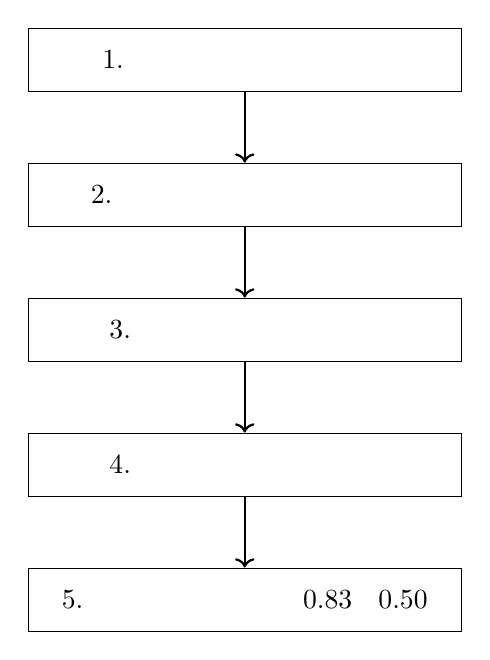
\begin{tikzpicture}[node distance=9mm, process/.style={draw, align=center, minimum width=55mm, minimum height=8mm}, arrow/.style={->, thick}]
\node[process] (a) {1. Получение сообщения пользователя};
\node[process, below=of a] (b) {2. Построение векторного представления};
\node[process, below=of b] (c) {3. Поиск пяти ближайших обращений};
\node[process, below=of c] (d) {4. Агрегация оценок по категориям};
\node[process, below=of d] (e) {5. Выбор сценария по порогам 0.83 и 0.50};
\draw[arrow] (a) -- (b);
\draw[arrow] (b) -- (c);
\draw[arrow] (c) -- (d);
\draw[arrow] (d) -- (e);
\end{tikzpicture}
\caption{Последовательность обработки пользовательского обращения}
\label{fig:request-sequence}
\end{figure}

В итоге управление диалоговым сценарием выполняет роль связующего слоя
между архитектурой системы и пользовательским взаимодействием. Оно
определяет, когда нужно выполнить поиск, когда можно вывести результат,
когда требуется выбор пользователя, а когда необходимо продолжить
диалог. Такой подход позволяет повысить надежность маршрутизации и
сделать работу системы более удобной для пользователя. Дальнейшее
качество этого сценария во многом зависит от модуля векторизации и
семантического поиска, который рассматривается в следующем подразделе.

\subsection{Модуль векторизации
текстов}

Модуль векторизации текстов отвечает за преобразование пользовательского
обращения в форму, пригодную для семантического поиска. В рамках системы
Service Desk ЦФТ пользователь отправляет сообщение в свободной форме, а
система должна сопоставить его с ранее обработанными тикетами. Для этого
текст обращения переводится в векторное представление, после чего по этому вектору
выполняется поиск ближайших объектов в векторной базе.

Необходимость такого модуля связана с особенностями обращений
пользователей. В системе существует несколько сотен категорий работ, при
этом распределение исторических обращений по ним является
несбалансированным. Часть категорий имеет большое количество примеров, а
часть представлена единичными заявками. В таких условиях прямое обучение
обычного многоклассового классификатора затруднено, поскольку модель
может хорошо работать только на часто встречающихся категориях и хуже
обрабатывать редкие классы. Поэтому в проекте был выбран подход,
основанный на поиске похожих исторических тикетов, а не на прямом
предсказании категории по фиксированному списку классов.

На вход модуль получает текст пользовательского сообщения. Это сообщение
рассматривается как новый тикет, который необходимо сопоставить с уже
имеющимися примерами. Далее текст передается в модель векторизации. В
проекте для этой задачи используется модель семейства E5,
предназначенная для построения текстовых векторное представление-представлений. На
уровне программной реализации модуль не решает задачу диалога и не
выбирает итоговый ответ пользователю. Его задача ограничена построением
вектора и подготовкой данных для последующего поиска.

После построения векторное представление выполняется обращение к векторной базе
данных. Векторная база хранит ранее подготовленные представления
исторических тикетов. Каждый такой тикет связан с метаданными, среди
которых важную роль играет поле категории работ. Категория работ
описывается как уникальный идентификатор заявки, хранящийся в метаданных
тикета. За счет этого результат поиска можно связать не только с похожим
текстом, но и с конкретной категорией, которая использовалась при
обработке исторического обращения.

Поиск в векторной базе возвращает набор ближайших тикетов и значения
расстояния или близости до них. Эти данные не являются итоговым
результатом для пользователя. Пользователю не нужно видеть список
похожих исторических заявок, ему нужна подходящая категория работ и
инструкция по дальнейшим действиям. Поэтому после поиска выполняется
преобразование найденных тикетов в категории-кандидаты. Если несколько
близких тикетов относятся к одной и той же категории, это усиливает
оценка результата в данном варианте. Если же ближайшие тикеты
распределены между разными категориями, результат считается менее
однозначным.

Ключевой задачей после поиска является агрегация результатов. Ранний
вариант системы опирался на категорию ближайшего тикета, что делало
поведение неустойчивым: один случайный ближайший пример мог определять
весь ответ. В ходе доработки был добавлен механизм агрегации нескольких
найденных тикетов. При таком подходе система учитывает не только самый
близкий объект, но и группу релевантных результатов. Для каждой
категории оценивается, сколько связанных с ней тикетов найдено и
насколько близко они расположены к запросу пользователя. На основе этого
формируется оценка результата, которая затем используется в диалоговой
логике.

Работу модуля можно представить как последовательность этапов. Сначала
текст запроса нормализуется в том виде, в котором его может обработать
модель векторизации. Затем строится векторное представление. После этого векторное представление
передается в векторную базу, где выполняется поиск ближайших
исторических тикетов. Найденные результаты возвращаются вместе с
метаданными и оценками близости. Далее данные группируются по категориям
работ, и для каждой категории формируется итоговая оценка. Результатом
работы модуля является не один текстовый ответ, а структурированный
набор категорий-кандидатов, который передается в управляющую логику
системы.

Основные функции модуля представлены в таблице 2.5.

\Needspace{8\baselineskip}
\textbf{Таблица 2.5 - Основные функции модуля векторизации текстов}

\begin{longtable}[]{@{}|
  >{\raggedright\arraybackslash}p{(\columnwidth - 2\tabcolsep) * \real{0.3234}}|
  >{\raggedright\arraybackslash}p{(\columnwidth - 2\tabcolsep) * \real{0.6766}}|@{}}
\hline
\begin{minipage}[t]{\linewidth}\raggedright
\TableHead{Функция}
\end{minipage} & \begin{minipage}[t]{\linewidth}\raggedright
\TableHead{Содержание}
\end{minipage} \\ \hline
\endhead
\begin{minipage}[t]{\linewidth}\raggedright
Получение пользовательского запроса
\end{minipage} & \begin{minipage}[t]{\linewidth}\raggedright
Прием текста обращения от основного сервиса
\end{minipage} \\ \hline
\begin{minipage}[t]{\linewidth}\raggedright
Построение векторное представление
\end{minipage} & \begin{minipage}[t]{\linewidth}\raggedright
Преобразование текста в числовое векторное представление
\end{minipage} \\ \hline
\begin{minipage}[t]{\linewidth}\raggedright
Поиск похожих тикетов
\end{minipage} & \begin{minipage}[t]{\linewidth}\raggedright
Обращение к векторной базе и получение ближайших исторических обращений
\end{minipage} \\ \hline
\begin{minipage}[t]{\linewidth}\raggedright
Извлечение метаданных
\end{minipage} & \begin{minipage}[t]{\linewidth}\raggedright
Получение категорий работ, связанных с найденными тикетами
\end{minipage} \\ \hline
\begin{minipage}[t]{\linewidth}\raggedright
Агрегация результатов
\end{minipage} & \begin{minipage}[t]{\linewidth}\raggedright
Группировка найденных тикетов по категориям работ
\end{minipage} \\ \hline
\begin{minipage}[t]{\linewidth}\raggedright
Расчет оценки результата
\end{minipage} & \begin{minipage}[t]{\linewidth}\raggedright
Формирование оценки, показывающей надежность найденной категории
\end{minipage} \\ \hline
\begin{minipage}[t]{\linewidth}\raggedright
Передача результата
\end{minipage} & \begin{minipage}[t]{\linewidth}\raggedright
Возврат категорий-кандидатов в основной сервис обработки
\end{minipage} \\ \hline
\end{longtable}

Важной особенностью модуля является его отделение от логики принятия
итогового решения. Модуль векторизации не определяет, какой сценарий
будет показан пользователю: одна категория, несколько вариантов или
уточняющий вопрос. Он предоставляет только результаты семантического
поиска и оценки, необходимые для принятия такого решения. Это разделение
делает архитектуру более управляемой: качество поиска можно улучшать
отдельно от пользовательского интерфейса и логики диалога.

Отдельно следует отметить связь модуля с исследовательской частью
работы. В текущей разделе модуль рассматривается с точки зрения его
прикладного назначения в составе веб-сервиса. Здесь важно показать,
какую функцию он выполняет в конвейер обработки обращения. Подробное
математическое описание модели E5, механизма формирования векторные представления текста, базового агрегирования и его модификации вынесено в третью раздел.
Такое разделение позволяет во втором разделе сосредоточиться на
программной роли модуля, а в третьей - на исследовании качества самой
модели векторизации.

В итоге модуль векторизации текстов выполняет роль связующего слоя между
свободным пользовательским сообщением и накопленной историей обращений.
Он позволяет искать не точные совпадения слов, а похожие по смыслу
тикеты, после чего переводит результаты поиска в набор
категорий-кандидатов. За счет этого система получает основу для
дальнейшего выбора сценария обработки: однозначного вывода одной
категории, предложения нескольких вариантов или перехода к уточнению
запроса.

\subsection{Модуль уточняющих
вопросов}

Модуль уточняющих вопросов используется в тех случаях, когда исходного
сообщения пользователя недостаточно для однозначного выбора категории
обращения. В системе Service Desk ЦФТ пользователь может отправить
короткий или неоднозначный запрос, например без указания конкретной
системы, типа доступа, ошибки или контекста выполнения операции. В такой
ситуации автоматический выбор одной категории может привести к неверной
маршрутизации, поэтому система должна продолжить диалог и получить
дополнительные сведения.

Назначение модуля состоит не в самостоятельной маршрутизации обращения,
а в поддержке диалогового сценария. Он подключается после этапа
семантического поиска, если найденные исторические тикеты не позволяют
надежно определить одну категорию. Управляющая логика передает в модуль
исходный запрос пользователя и сведения о неопределенности результата,
после чего формируется уточняющий вопрос. Ответ пользователя затем
возвращается в основной конвейер обработки и используется для повторного
поиска.

Такой подход позволяет не завершать обработку при низкой оценке и
не выдавать случайный результат. Вместо этого система переводит
неоднозначную ситуацию в управляемый диалог. Например, если пользователь
пишет только «нужен доступ», система может уточнить, к какой системе или
ресурсу требуется доступ. После получения ответа запрос становится более
информативным, и вероятность корректного выбора категории повышается.

В рамках архитектуры модуль уточняющих вопросов является вспомогательным
компонентом. Он не заменяет модуль векторизации, базу исторических
обращений или базу знаний, а используется только в тех сценариях, где
требуется дополнительное взаимодействие с пользователем. Это важно для
управляемости системы: итоговое решение по-прежнему принимается на
основе поиска похожих обращений и оценки результата, а языковая модель
применяется для формирования понятного вопроса.

Основные функции модуля представлены в таблице 2.6.

\Needspace{8\baselineskip}
\textbf{Таблица 2.6 - Основные функции модуля уточняющих вопросов}

\begin{longtable}[]{@{}|
  >{\raggedright\arraybackslash}p{(\columnwidth - 2\tabcolsep) * \real{0.2605}}|
  >{\raggedright\arraybackslash}p{(\columnwidth - 2\tabcolsep) * \real{0.7395}}|@{}}
\hline
\begin{minipage}[t]{\linewidth}\raggedright
\TableHead{Функция}
\end{minipage} & \begin{minipage}[t]{\linewidth}\raggedright
\TableHead{Содержание}
\end{minipage} \\ \hline
\endhead
\begin{minipage}[t]{\linewidth}\raggedright
Получение контекста
\end{minipage} & \begin{minipage}[t]{\linewidth}\raggedright
Прием исходного запроса и данных о неопределенности результата
\end{minipage} \\ \hline
\begin{minipage}[t]{\linewidth}\raggedright
Формирование вопроса
\end{minipage} & \begin{minipage}[t]{\linewidth}\raggedright
Генерация уточняющего вопроса на естественном языке
\end{minipage} \\ \hline
\begin{minipage}[t]{\linewidth}\raggedright
Поддержка диалога
\end{minipage} & \begin{minipage}[t]{\linewidth}\raggedright
Продолжение сценария при недостатке информации
\end{minipage} \\ \hline
\begin{minipage}[t]{\linewidth}\raggedright
Возврат в конвейер
\end{minipage} & \begin{minipage}[t]{\linewidth}\raggedright
Использование ответа пользователя для повторной обработки запроса
\end{minipage} \\ \hline
\end{longtable}

В итоге модуль уточняющих вопросов повышает качество обслуживания
системы к неполным и неоднозначным обращениям. Он позволяет сохранить
качество взаимодействия с пользователем, не заставляя систему выбирать
категорию при неопределенном ответе. Благодаря этому чат-бот работает
не как жесткий классификатор, а как диалоговая система, способная
уточнять смысл запроса перед финальной маршрутизацией.

\subsection{Пользовательский интерфейс и
веб-сервер}

Пользовательский интерфейс реализован как внешняя часть системы, через
которую пользователь взаимодействует с чат-ботом Service Desk ЦФТ. Он
обеспечивает ввод обращения, отображение истории сообщений, вывод
результатов обработки, выбор подходящей категории и просмотр инструкции
по дальнейшим действиям. Интерфейс построен в формате диалога, поэтому
пользователь работает с системой привычным способом: отправляет
сообщение, получает ответ, выбирает вариант или продолжает уточнение
запроса.

В интерфейсе реализован ввод обращения в свободной форме. Пользователю
не требуется самостоятельно искать нужную категорию в большом дереве
заявок. Он описывает проблему обычным текстом, а система выполняет
первичную обработку запроса на серверной стороне. Такое решение снижает
сложность взаимодействия, поскольку пользователь не обязан знать
внутреннюю структуру категорий работ.

Для отображения результата реализовано несколько сценариев. Если система
однозначно определила категорию, интерфейс выводит ее пользователю вместе
с инструкцией. Если найдено несколько близких вариантов, они
отображаются как элементы выбора. Пользователь выбирает подходящую
категорию, после чего система показывает соответствующую справочную
информацию. Если исходного сообщения недостаточно, интерфейс отображает
уточняющий вопрос и позволяет продолжить диалог без перезапуска
сценария.

Отдельно реализован вывод информации по выбранной категории.
Пользователь получает не только название категории, но и путь в дереве
заявок, описание и гайд. Это делает результат прикладным: система не
просто сообщает найденный вариант, а помогает пользователю правильно
оформить дальнейшее обращение. За счет этого интерфейс выполняет роль не
только чат-окна, но и навигационного инструмента по процессу создания
заявки.

Веб-серверная часть реализует связь пользовательского интерфейса с
остальными компонентами системы. Интерфейс передает пользовательские
сообщения и действия на серверную сторону, а сервер возвращает
структурированный ответ для отображения. Семантический поиск, получение
инструкций, работа с историей и обработка сценариев выполняются на
стороне серверных компонентов, поэтому интерфейс остается отделенным от
основной логики маршрутизации.

Взаимодействие между интерфейсом и серверной частью реализовано как
многошаговый диалог. В рамках одной сессии пользователь отправляет
исходный запрос, отвечает на уточнение, выбирает предложенный вариант,
просматривает инструкцию и при необходимости продолжает взаимодействие.
Серверная часть сохраняет состояние сценария и корректно различает типы
действий пользователя: новое сообщение, выбор категории, ответ на
уточнение или оценку результата.

В системе реализовано сохранение истории диалогов. Пользователь видит
предыдущие сообщения и ответы системы, а также может вернуться к ранее
начатому взаимодействию. Сохранение истории вынесено в серверный слой и
не зависит только от состояния страницы в браузере. Это позволяет
восстановить диалог после обновления интерфейса и использовать
накопленные данные для анализа качества работы системы.

Также реализован механизм пользовательской обратной связи. После
получения результата пользователь может оценить ответ системы. Эти
оценки сохраняются вместе с историей взаимодействия и используются как
источник данных для последующего анализа. Такой механизм важен для
развития сервиса, поскольку позволяет выявлять случаи некорректной
маршрутизации, неудобные сценарии и категории, по которым система чаще
требует доработки.

Основные реализованные UX-функции интерфейса представлены в таблице 2.7.

\Needspace{8\baselineskip}
\textbf{Таблица 2.7 - Реализованные UX-функции пользовательского
интерфейса}

\begin{longtable}[]{@{}|
  >{\raggedright\arraybackslash}p{(\columnwidth - 2\tabcolsep) * \real{0.2140}}|
  >{\raggedright\arraybackslash}p{(\columnwidth - 2\tabcolsep) * \real{0.7860}}|@{}}
\hline
\begin{minipage}[t]{\linewidth}\raggedright
\TableHead{Функция}
\end{minipage} & \begin{minipage}[t]{\linewidth}\raggedright
\TableHead{Реализация}
\end{minipage} \\ \hline
\endhead
\begin{minipage}[t]{\linewidth}\raggedright
Свободный ввод обращения
\end{minipage} & \begin{minipage}[t]{\linewidth}\raggedright
Пользователь вводит проблему обычным текстом без ручного выбора
категории
\end{minipage} \\ \hline
\begin{minipage}[t]{\linewidth}\raggedright
Диалоговый формат
\end{minipage} & \begin{minipage}[t]{\linewidth}\raggedright
Сообщения пользователя и ответы системы отображаются в виде чата
\end{minipage} \\ \hline
\begin{minipage}[t]{\linewidth}\raggedright
Вывод результата
\end{minipage} & \begin{minipage}[t]{\linewidth}\raggedright
Интерфейс показывает найденную категорию и связанную с ней инструкцию
\end{minipage} \\ \hline
\begin{minipage}[t]{\linewidth}\raggedright
Выбор из вариантов
\end{minipage} & \begin{minipage}[t]{\linewidth}\raggedright
При наличии нескольких подходящих категорий пользователь выбирает нужный
вариант
\end{minipage} \\ \hline
\begin{minipage}[t]{\linewidth}\raggedright
Уточнение запроса
\end{minipage} & \begin{minipage}[t]{\linewidth}\raggedright
При недостатке информации пользователь получает дополнительный вопрос и
продолжает диалог
\end{minipage} \\ \hline
\begin{minipage}[t]{\linewidth}\raggedright
История чатов
\end{minipage} & \begin{minipage}[t]{\linewidth}\raggedright
Предыдущие сообщения и ответы системы сохраняются и отображаются в
интерфейсе
\end{minipage} \\ \hline
\begin{minipage}[t]{\linewidth}\raggedright
Обратная связь
\end{minipage} & \begin{minipage}[t]{\linewidth}\raggedright
Пользователь оценивает результат работы системы
\end{minipage} \\ \hline
\begin{minipage}[t]{\linewidth}\raggedright
Голосовой ввод
\end{minipage} & \begin{minipage}[t]{\linewidth}\raggedright
Пользователь может передать обращение в голосовом формате, после чего
оно обрабатывается как текстовый запрос
\end{minipage} \\ \hline
\end{longtable}

Голосовой ввод реализован как дополнительный пользовательский сценарий.
Пользователь передает обращение в аудиоформате, после чего оно
преобразуется в текст и поступает в основной конвейер обработки.
Дальнейшая логика не отличается от обычного текстового обращения:
система выполняет семантический поиск, вычисляет оценку результата
и формирует ответ в интерфейсе.

Веб-сервер также реализует работу с пользовательскими данными. Он
отвечает за сохранение истории чатов, восстановление предыдущих диалогов
и передачу пользовательской оценки. Благодаря этому интерфейс не хранит
критически важное состояние только на клиентской стороне. Основные
данные взаимодействия сохраняются на сервере, что повышает надежность
пользовательского сценария.

В итоге пользовательский интерфейс и веб-сервер образуют прикладной слой
системы. Интерфейс предоставляет пользователю понятный диалоговый способ
работы с чат-ботом, а веб-сервер связывает пользовательские действия с
основным конвейером обработки обращений. Реализованное решение скрывает
сложность внутренней архитектуры и представляет ее в простой форме:
пользователь отправляет обращение, получает результат, выбирает вариант,
уточняет запрос или оценивает ответ системы.

\subsection{Выводы по разделу 2}

Во втором разделе была рассмотрена программная реализация системы
маршрутизации обращений Service Desk ЦФТ. Были сформулированы основные
требования к системе, связанные с обработкой пользовательских запросов,
поиском подходящей категории работ, поддержкой диалогового сценария,
выводом справочной информации и сохранением истории взаимодействия.

Было показано, что разрабатываемая система построена как
последовательный конвейер обработки обращения. Пользователь вводит
сообщение в свободной форме, после чего система определяет текущее
состояние диалога, выполняет семантический поиск по историческим
обращениям, агрегирует найденные результаты по категориям и выбирает
дальнейший сценарий взаимодействия. В зависимости от оценки результата
результата система выводит одну категорию, предлагает несколько
вариантов или продолжает диалог с пользователем.

Отдельно была рассмотрена логика управления диалоговым сценарием. В
отличие от одношагового классификатора, разработанная система учитывает
состояние взаимодействия с пользователем. Это позволяет корректно
обрабатывать не только первичный запрос, но и выбор категории, ответ на
уточнение, просмотр инструкции и оценку результата. Такой подход делает
работу системы более устойчивой к неполным и неоднозначным
формулировкам.

Также был описан модуль векторизации текстов, который выполняет
преобразование пользовательского обращения в векторное представление и обеспечивает
поиск похожих исторических тикетов. Результаты поиска используются не
напрямую, а после агрегации по категориям работ. За счет этого система
получает не отдельный похожий пример, а набор категорий-кандидатов с
агрегированными оценками. Это позволяет применять семантический поиск как
основу для маршрутизации обращений.

Кроме того, была рассмотрена реализация пользовательского интерфейса и
веб-серверной части. Интерфейс предоставляет пользователю диалоговый
способ взаимодействия с системой: ввод обращения, получение результата,
выбор из нескольких категорий, просмотр инструкции, продолжение
уточнения и оценку ответа. Веб-серверная часть связывает
пользовательские действия с основным конвейером обработки и обеспечивает
сохранение истории диалогов.

В результате во втором разделе была описана прикладная часть разработанной
системы: от постановки задачи и архитектуры до основных пользовательских
сценариев. Реализованное решение позволяет автоматизировать первичную
обработку обращений, снизить зависимость от ручного выбора категории и
представить пользователю результат в понятной форме. При этом качество
работы всей системы во многом зависит от того, насколько точно модуль
векторизации сопоставляет пользовательский запрос с историческими
обращениями. Поэтому в следующей разделе рассматривается математическое
обеспечение модели векторных представлений и ее модификация, направленная на
повышение качества семантического поиска.

\clearpage
\section{Исследование и доработка модели векторизации запросов}

\subsection{Формализация задачи семантического поиска}

В разрабатываемой системе задача выбора категории работ для
пользовательского обращения рассматривается как задача семантического
поиска. Такой подход отличается от прямой многоклассовой классификации:
система не пытается сразу предсказать один класс из заранее заданного
множества, а сначала сопоставляет новое обращение с ранее обработанными
обращениями. Затем на основе найденных похожих примеров формируется
ранжированный список категорий-кандидатов.

Пусть имеется множество исторических обращений:

\begin{equation}\mathcal{D}=\{d_1,d_2,\ldots,d_n\}.\end{equation}

Каждому обращению \(d_{i}\) соответствует категория работ \(c_{i}\) из
множества категорий:

\begin{equation}\mathcal{C}=\{c_1,c_2,\ldots,c_m\}.\end{equation}

Новое пользовательское обращение обозначим как \(q\). Требуется найти
такие элементы множества \(D\), которые наиболее близки к запросу \(q\)
по смыслу, а затем определить категорию работ, наиболее соответствующую
текущему обращению. В отличие от поиска по ключевым словам, здесь важна
не только лексическая близость текстов, но и их смысловое сходство. Это
важно для пользовательских обращений, так как одна и та же проблема
может быть сформулирована разными словами.

Для выполнения семантического поиска каждый текст преобразуется в
векторное представление. Обозначим модель векторизации как
\(f_{\omega}\) . Тогда векторное представление пользовательского запроса можно
записать следующим образом:

\begin{equation}\symbfit{e}(q)=f_{\omega}(q).\label{eq:query-vector}\end{equation}

Для исторического обращения:

\begin{equation}\symbfit{e}(d_i)=f_{\omega}(d_i),\quad d_i\in\mathcal{D}.\label{eq:doc-vector}\end{equation}

В этих выражениях \(e_{q}\) и \(e_{i}\) являются плотными векторными
представлениями текстов, а \(\omega\) обозначает параметры модели
векторизации. Основное требование к такой модели состоит в том, чтобы
обращения, близкие по смыслу и относящиеся к одной категории работ,
располагались в векторном пространстве ближе друг к другу, чем обращения
разных категорий.

Для сравнения векторов используется мера близости. В задачах поиска по
векторным представлениям часто применяется косинусная близость, которая
оценивает угол между двумя векторами:

\begin{equation}s(q,d_i)=\frac{(\symbfit{e}(q),\symbfit{e}(d_i))}{\|\symbfit{e}(q)\|_2\|\symbfit{e}(d_i)\|_2}.\label{eq:cosine}\end{equation}

Чем больше значение \(sim\left( e_{q},e_{i} \right)\), тем более
близкими считаются пользовательский запрос и историческое обращение.
После вычисления близости между запросом и элементами корпуса
формируется ранжированный список результатов:

\begin{equation}R(q)=\operatorname{sort}_{d_i\in\mathcal{D}}\bigl(s(q,d_i)\bigr).\label{eq:ranking}\end{equation}

Первые элементы этого списка образуют выдачу из первых K результатов:

\begin{equation}\operatorname{TopK}(q)=\{d_{(1)},d_{(2)},\ldots,d_{(K)}\},\quad K=5.\end{equation}

Здесь \(K\) задает число ближайших исторических обращений, которые
учитываются при дальнейшем выборе категории работ. Использование первых K результатов
важно, поскольку один ближайший пример не всегда надежно отражает смысл
пользовательского запроса. В условиях большого числа категорий и
неоднородных данных отдельное историческое обращение может оказаться
близким случайно. Поэтому более устойчивым является анализ группы
ближайших результатов.

После получения первых K результатов выполняется переход от найденных обращений к категориям работ. Каждому найденному обращению сопоставляется категория, затем для каждой категории вычисляется агрегированная оценка по формуле~\eqref{eq:category-score}. Основная категория-кандидат выбирается по правилу~\eqref{eq:argmax-category}.

Для категории c можно задать совокупную оценку на основе близости
найденных обращений:

\begin{equation}S(c,q)=\sum_{d\in\operatorname{TopK}(q):\,c(d)=c}\frac{1}{1+\delta(q,d)}.\label{eq:category-score}\end{equation}

Значение \(S(c,q)\) показывает, насколько сильно категория c
представлена среди ближайших результатов. После вычисления таких оценок
для всех категорий-кандидатов формируется ранжированный список
категорий:

\begin{equation}C_q=\operatorname{sort}_{c\in\mathcal{C}}\bigl(S(c,q)\bigr).\label{eq:category-ranking}\end{equation}

Категория с наибольшей оценкой является основной кандидатной категорией.
Однако итоговый сценарий работы системы зависит не только от первого
места в списке, но и от оценки результата. Если первая
категория существенно превосходит остальные, система может вывести ее
пользователю как наиболее вероятную. Если несколько категорий имеют
близкие оценки, пользователь получает список вариантов. Если оценки
низкие или распределены неустойчиво, система переходит к уточнению
запроса.

Основная категория-кандидат выбирается по правилу максимума агрегированной оценки:

\begin{equation}c^\ast(q)=\arg\max_{c\in\mathcal{C}} S(c,q).\label{eq:argmax-category}\end{equation}

Здесь \(c^\ast(q)\) является категорией с наибольшей агрегированной оценкой. При низкой оценке результата система не выдает единственный результат, поскольку это увеличивает риск ошибочной маршрутизации.

В рамках данной работы такая постановка задачи является наиболее
подходящей по нескольким причинам. Во-первых, исторические обращения уже
содержат практические примеры реальных пользовательских запросов и
связанных с ними категорий работ. Во-вторых, число категорий велико, а
распределение данных по категориям неравномерно, поэтому прямое обучение
классификатора может быть нестабильным для редких категорий. В-третьих,
пользователю может быть полезен не только один ответ, но и несколько
наиболее вероятных вариантов, если система не уверена в результате.

С точки зрения дальнейшего исследования ключевым элементом описанной
схемы является модель векторизации \(f_{\omega}\). Именно она определяет
расположение обращений в пространстве векторных представлений и, следовательно, влияет
на порядок объектов в выдаче из первых K результатов. Если векторное представление построено неудачно,
похожие по смыслу обращения могут оказаться далеко друг от друга, а
обращения разных категорий - слишком близко. В этом случае даже
корректная агрегация результатов не позволит надежно выбрать категорию
работ.

Именно поэтому дальнейшая часть раздела посвящена модели построения
векторные представления текста. Сначала рассматриваются математические основы
базовой модели E5 и стандартного способа формирования вектора всего
текста. Затем анализируются ограничения усреднение токенных представлений и предлагается
модификация механизма агрегирования, направленная на более точное выделение
информативных токенов при построении векторного представления пользовательского
обращения.

\subsection{Векторные представления текста}

Для выполнения семантического поиска пользовательское обращение
необходимо представить в виде числового вектора. Такое представление
должно сохранять основное содержание текста и позволять сравнивать
обращение с историческими заявками. В рассматриваемой работе для этой
цели используется модель векторизации
intfloat/multilingual-e5-large-instruct, относящаяся к семейству E5.
Данная модель применяется для построения плотных текстовых
представлений, которые далее используются при поиске похожих обращений.

В общем виде процесс векторизации можно описать как отображение текста в
векторное пространство. Пусть \(x\) обозначает текст обращения,
\(f_{\omega}\)- модель векторизации с параметрами \(\omega\), а \(e\) -
итоговое векторное представление текста. Тогда преобразование записывается следующим
образом:

\begin{equation}\symbfit{e}(x)=f_{\omega}(x).\end{equation}

Смысл такого отображения заключается в том, что тексты, близкие по
содержанию, должны располагаться близко друг к другу в общем векторном
пространстве. Если пользовательское обращение и историческая заявка
описывают одну и ту же проблему или относятся к одной категории работ,
расстояние между их векторными представлениями должно быть меньше, чем
расстояние до обращений других категорий. Поэтому качество модели
векторизации напрямую влияет на качество поиска похожих обращений и
последующей маршрутизации.

Для корректного сопоставления пользовательских запросов и исторических
заявок они должны кодироваться одной и той же моделью. Это означает, что
новое обращение пользователя и ранее сохраненные обращения отображаются
в одно и то же пространство признаков. Благодаря этому их можно
сравнивать с помощью одной меры близости, например косинусной близости.
Такой подход позволяет работать не с исходными строками текста, а с их
числовыми представлениями.

Перед подачей текста в модель выполняется токенизация. Исходное
обращение разбивается на последовательность токенов. Токенами могут быть
слова, части слов, знаки препинания и специальные элементы, используемые
моделью. Токенизированный текст можно записать следующим образом:

\begin{equation}x=[t_1,t_2,\ldots,t_m].\end{equation}

где \(t_{i}\) - i-й токен входного текста, \(m\) - длина
токенизированной последовательности.

После токенизации последовательность токенов поступает в модель-кодировщик.
Кодировщик строит контекстные представления токенов, то есть учитывает не
только сам токен, но и его окружение во входном тексте. Это особенно
важно для пользовательских обращений, поскольку смысл отдельных слов
может зависеть от контекста. Например, одно и то же слово в разных
обращениях может указывать на разные действия, системы или типы проблем.

Работу модели-кодировщика можно записать так:

\begin{equation}\symbfit{H}=F_{\beta}(t_1,t_2,\ldots,t_m).\end{equation}

где \(F_{\beta}\) - кодировщик с параметрами \(\omega\), а \(H\) -
результат его работы. Важно, что результатом кодировщика является не один
вектор всего текста, а последовательность скрытых состояний:

\begin{equation}\symbfit{H}=[\symbfit{h}_1,\symbfit{h}_2,\ldots,\symbfit{h}_m].\end{equation}

Здесь \(\symbfit{h}_i\) обозначает скрытое векторное представление токена
\(t_i\). Каждое такое представление содержит информацию о токене с
учетом его позиции и контекста внутри обращения.

Для задачи семантического поиска одной последовательности токенных
представлений недостаточно. Необходимо получить один вектор, описывающий
весь текст обращения. Такой итоговый вектор называется векторное представление текста. Несмотря на название, векторное представление текста может описывать не
только одно предложение, но и пользовательский запрос, описание заявки
или другой короткий текст. Именно этот вектор далее используется для
сравнения текущего обращения с историческими обращениями.

Переход от набора токенных представлений к одному вектору выполняется с
помощью механизма агрегирования. В общем виде агрегирование можно записать следующим
образом:

\begin{equation}\symbfit{z}=P(\symbfit{H},\symbfit{a}).\label{eq:pooling-general}\end{equation}

где \(z\) - промежуточный вектор всего текста, \(H\) -
последовательность скрытых состояний токенов, a - маска внимания.

Маска внимания необходима из-за того, что тексты имеют разную длину. При
пакетной обработке короткие последовательности дополняются специальными
padding-токенами. Эти токены не содержат смысловой информации и не
должны влиять на итоговое векторное представление. Маска внимания показывает, какие
позиции соответствуют реальным токенам исходного текста, а какие были
добавлены только для выравнивания длины последовательности.

После агрегирование применяется нормализация итогового вектора:

\begin{equation}\symbfit{e}(x)=\frac{\symbfit{z}(x)}{\|\symbfit{z}(x)\|_2}.\end{equation}

Нормализация переводит вектор к единичной длине. Это удобно для
дальнейшего сравнения векторное представлениеов, поскольку в задачах
семантического поиска важно прежде всего направление вектора, а не его
абсолютная длина. После нормализации близость между текстами может
оцениваться через косинусную близость или скалярное произведение
нормализованных векторов.

В рассматриваемой задаче векторное представление текста выполняет роль компактного
числового описания обращения. Он должен сохранять признаки, важные для
выбора категории работ: объект обращения, тип проблемы, действие
пользователя, упоминание системы или сервиса, а также общий смысл
запроса. При этом векторное представление не должен чрезмерно зависеть от
второстепенных слов и шаблонных фраз, которые часто встречаются в
обращениях, но слабо помогают отличать одну категорию от другой.

Качество итогового векторного представления текста определяется двумя основными
факторами. Первый фактор - качество модели-кодировщика, которая строит
контекстные представления токенов. Второй фактор - способ агрегации этих
токенных представлений в один вектор текста. Даже если кодировщик формирует
информативные скрытые состояния, итоговое векторное представление может потерять часть
значимой информации при неудачном агрегировании. Поэтому механизм агрегирования
является важной частью модели векторизации.

Для системы маршрутизации обращений это особенно существенно.
Пользовательские запросы часто бывают короткими, неполными или
сформулированными в свободной форме. Правильная категория работ может
зависеть от одного или нескольких ключевых токенов, например названия
системы, типа доступа или конкретной ошибки. Если при построении
векторное представление текста все токены учитываются одинаково, вклад таких
информативных элементов может быть ослаблен общими словами и шаблонными
фрагментами текста.

Таким образом, модель E5 используется как основа для построения
векторных представлений обращений, а векторное представление текста является
основным объектом, с которым работает семантический поиск.
Пользовательский запрос и исторические заявки кодируются одной моделью,
после чего сравниваются в общем векторном пространстве. При этом
качество поиска зависит не только от модели-кодировщика, но и от способа
получения одного векторного представления из последовательности токенных
представлений. В следующем подразделе рассматривается базовый способ
такой агрегации - усреднение токенных представлений, а также его ограничения применительно к
задаче маршрутизации обращений.

\subsection{Базовое усреднение токенных представлений и его
ограничения}

После получения контекстных векторов \(\symbfit{h}_i\) для токенов входного обращения
необходимо объединить их в единое представление текста. Для этого часто
используют метод усреднение токенных представлений -- усреднение по всем реальным токенам.
При пакетной обработке различной длины текстов задействуется маска
внимания \(a\), где \(a_i=1\) для реального токена и \(a_i=0\) для padding. В
таком случае усреднение токенных представлений с учётом маски определяется как

\begin{equation}\symbfit{v}_{mean}(x)=\frac{\sum_{i=1}^{m} a_i\symbfit{h}_i}{\sum_{i=1}^{m}a_i}.\label{eq:mean-pooling}\end{equation}

Усреднение токенных представлений обладает необходимой инвариантностью к padding-токенам
(благодаря маске) и сохраняет пропорции признаков при разных длинах
текста. Однако на практике этот подход сталкивается с рядом ограничений.
Во-первых, в усреднении участвуют все токены с одинаковым весом. Это
означает, что часто встречающиеся служебные или шаблонные слова
(«помогите», «ошибка», «не могу» и подобные) вносят равный вклад с
редкими, но информативными терминами. Например, в запросе «Ошибка 403
доступа» слова «ошибка» и «доступ» (очень частотные в обращениях)
уменьшают относительную значимость конкретного кода «403» и наоборот. В
результате итоговое векторное представление может стать размытым и менее
чувствительным к сути запроса.

Во-вторых, короткие обращения особенно уязвимы к шуму. Если запрос
состоит из двух--трёх токенов (например, «Ошибка 403» или «Нет
доступа»), усреднение токенных представлений просто усреднит их представления. При этом
каждый токен оказывает сильное влияние на векторное представление. Если среди них
присутствует общеупотребительное слово, оно может выровнять
представления разных категорий. К примеру, запрос «Нет доступа»
встречается в множестве ситуаций: права могут быть разные, а тексты
практически не содержат различий. Среднее векторное представление таких коротких
сообщений зачастую оказывается неопределённым -- ему не хватает ключевых
слов для однозначной классификации.

Кроме того, усреднение токенных представлений не учитывает статистику токенов по всему
корпусу. В системах поддержки часто встречаются имена систем, проектов
или функций (например, «SAP», «Exchange», «файловая система»), которые
являются важным сигналом категории. Так как все токены равноправны,
распространённые слова («система», «доступ») получают такой же вес, как
редкие названия. Это снижает влияние специфических терминов и мешает
отличать похожие запросы. Наконец, если данные по категориям сильно
несбалансированы, векторное представление, усреднённый по токенам, может склоняться к
общим словам доминирующей группы. В результате при маршрутизации
обращений система может хуже различать редкие или нетипичные категории.

При разработке альтернативных методов агрегирование важно сохранить
положительные свойства mean-подхода: инвариантность к добавлению
padding-токенов, стабильность в сравнении коротких и длинных текстов и
чувствительность к действительно информативным словам. В общем виде
агрегирование можно обобщить, введя веса \(w_i\) для каждого токена. Тогда
итоговый вектор считается как

\begin{equation}\symbfit{v}_{w}(x)=\frac{\sum_{i=1}^{m} a_iw_i\symbfit{h}_i}{\sum_{i=1}^{m}a_iw_i}.\label{eq:weighted-pooling-general}\end{equation}

(при этом усреднение токенных представлений соответствует случаю \(w_i=a_i\)). После
агрегации вектор снова нормализуется. Вышеописанные
ограничения усреднение токенных представлений показывают необходимость модификации схемы
агрегации: нужно усилить вклад редких информативных токенов и уменьшить
влияние шаблонных слов. В следующем разделе будет рассмотрен вариант
TF-IDF-взвешенного агрегирования, который призван решить эти задачи и улучшить
качество векторного представления текста в системе маршрутизации обращений.

\subsection{TF-IDF-взвешенное агрегирование}

В рамках бакалаврской работы была выполнена модификация способа
формирования итогового векторного представления текста для пользовательского
обращения. Базовая схема усреднение токенных представлений усредняет скрытые состояния
токенов с одинаковым весом, из-за чего информативные элементы обращения
и частотные шаблонные слова участвуют в построении вектора одинаково.
Для задачи маршрутизации обращений это ограничение существенно,
поскольку категория работ часто определяется небольшим числом значимых
токенов: названием системы, типом ошибки, объектом доступа или
конкретным действием пользователя.

В модифицированной схеме итоговое векторное представление формируется как
TF-IDF-взвешенное среднее токенных представлений. При этом изменяется не
модель-кодировщик, а этап агрегации скрытых состояний. Кодировщик по-прежнему
формирует контекстные представления токенов, после чего каждому токену
назначается вес, зависящий от его частоты в текущем обращении и
распространенности в обучающем корпусе.

Пусть токенизированное обращение имеет вид:

\begin{equation}x=[t_1,t_2,\ldots,t_m].\label{eq:tokenized-query}\end{equation}

После обработки модель-кодировщик формирует последовательность скрытых
состояний:

\begin{equation}\symbfit{H}=[\symbfit{h}_1,\symbfit{h}_2,\ldots,\symbfit{h}_m].\end{equation}

где \(\symbfit{h}_i\) - скрытое состояние токена \(t_i\).

Для каждого токена вычисляется частота в текущем обращении:

\begin{equation}\operatorname{tf}(t,x)=\frac{n(t,x)}{|x|}.\label{eq:tf}\end{equation}

где \(n(t_i,x)\) - число вхождений токена \(t_i\) в обращение \(x\), \(m\) -
количество токенов, участвующих в обработке.

Обратная документная частота вычислялась по обучающему корпусу:

\begin{equation}\operatorname{idf}(t)=\ln\frac{N+1}{\operatorname{df}(t)+1}+1.\label{eq:idf}\end{equation}

где \(N\) - число обращений в обучающей выборке, \(\operatorname{df}(t_i)\) - число обращений
обучающей выборки, в которых встречается токен \(t_i\). IDF рассчитывался
только по обучающей части данных, чтобы значения весов не использовали
информацию из валидационной и тестовой выборок.

TF-IDF значение токена определяется как произведение локальной частоты и
обратной документной частоты:

\begin{equation}\operatorname{tfidf}(t,x)=\operatorname{tf}(t,x)\operatorname{idf}(t).\label{eq:tfidf}\end{equation}

В бакалаврской работе TF-IDF не заменяет полностью базовый вес токена, а
добавляется к нему через коэффициент \(\alpha\). Итоговый вес токена задается
формулой

\begin{equation}w_i(\alpha)=1+\alpha\operatorname{tfidf}(t_i,x).\label{eq:tfidf-weight}\end{equation}

Такой вид веса сохраняет связь с усреднением токенных представлений. Если \(\alpha=0\), то для
всех токенов получается \(w_i=1\), и схема совпадает с обычным
усреднением. При \(\alpha>0\) токены с более высоким TF-IDF
получают больший вклад в итоговое векторное представление. Поэтому модифицированное
агрегирование является обобщением усреднения токенных представлений, а не полностью отдельным
способом построения вектора.

С учетом маски внимания итоговое взвешенное среднее вычисляется
следующим образом:

\begin{equation}\symbfit{z}_{tfidf}(x)=\frac{\sum_{i=1}^{m}a_iw_i(\alpha)\symbfit{h}_i}{\sum_{i=1}^{m}a_iw_i(\alpha)}.\label{eq:tfidf-pooling}\end{equation}

где \(a_i\) - элемент маски внимания. Если токен относится к исходному
тексту, то \(a_i=1\); если позиция соответствует padding-токену, то
\(a_i=0\). За счет этого padding-токены не участвуют в агрегации и не искажают
итоговое представление обращения.

После взвешенного агрегирования выполняется нормализация итогового вектора:

\begin{equation}\symbfit{e}(x)=\frac{\symbfit{z}(x)}{\|\symbfit{z}(x)\|_2}.\end{equation}

Нормализованный вектор \(\symbfit{e}\) используется как векторное представление текста обращения.
Нормализация необходима для дальнейшего сравнения обращений в едином
векторном пространстве, поскольку при семантическом поиске важна
близость направлений векторных представлений.

Смысл выполненной модификации состоит в перераспределении вклада токенов
при построении векторное представление. Часто встречающиеся и слабо различающие токены
получают небольшой дополнительный вклад, поскольку их IDF ниже. Более
специфичные токены, характерные для отдельных категорий работ, получают
больший вес и сильнее влияют на направление итогового вектора.

Многие пользовательские сообщения содержат общие фразы, которые
встречаются в разных категориях: просьбы о доступе, указания на ошибку,
общие описания проблемы. При равномерном усреднении такие фрагменты
могут размывать вклад действительно значимых элементов.
TF-IDF-взвешенное агрегирование уменьшает этот эффект, поскольку итоговый
вектор сильнее зависит от доменно значимых токенов.

В рамках проекта коэффициент \(\alpha\) рассматривался как обучаемый параметр
механизма агрегирования. Это позволило не задавать силу влияния TF-IDF
вручную, а подобрать ее в процессе обучения на примерах обращений.
Обучение было направлено на то, чтобы обращения одной категории
располагались ближе друг к другу, а обращения разных категорий - дальше.
Тем самым TF-IDF-взвешенное агрегирование было связано не только со статистикой
корпуса, но и с целевой задачей семантического поиска.

Формально модифицированную модель можно записать как отображение:

\begin{equation}\symbfit{e}_{tfidf}(x)=f_{\beta,\alpha}(x).\label{eq:modified-model}\end{equation}

где \(\beta\) - параметры модели-кодировщика, а \(\alpha\) - параметр, управляющий
влиянием TF-IDF весов при агрегировании. В данной схеме кодировщик формирует
токенные представления, а модифицированное агрегирование определяет, какие
токены сильнее участвуют в построении итогового векторного представления текста.

В результате в проекте был изменен именно механизм перехода от токенных
представлений к вектору всего обращения. Это позволило сохранить общую
структуру модели E5 и адаптировать итоговое пространство векторных представлений к
данным службы поддержки. Дальнейшая оценка выполнялась путем сравнения
базовой схемы усреднения токенных представлений и модифицированной схемы TF-IDF-взвешенного
агрегирования по метрикам извлечения релевантной информации.

\subsection{Интеграция нового механизма агрегирования}

В предыдущих подразделах было показано, что модель векторизации
формирует последовательность токенных представлений, а итоговое векторное представление текста получается за счет механизма агрегирования. Следовательно,
модификация модели может быть выполнена не за счет изменения всего
кодировщика, а за счет изменения способа агрегации скрытых состояний
токенов. Такой подход сохраняет сильные стороны базовой модели E5 и
одновременно позволяет адаптировать итоговое представление текста к
предметной области обращений службы поддержки.

В базовой схеме модель векторизации можно представить как композицию
трех этапов: построение токенных представлений, их агрегация и
нормализация итогового вектора. Пусть входное обращение обозначается как
x, кодировщик с параметрами \(\beta\) формирует последовательность скрытых
состояний:

\begin{equation}\symbfit{H}=F_{\beta}(x).\end{equation}

где

\begin{equation}\symbfit{H}=[\symbfit{h}_1,\symbfit{h}_2,\ldots,\symbfit{h}_m].\end{equation}

Здесь \(\symbfit{h}_i\) - скрытое состояние \(i\)-го токена, а \(m\) - длина
токенизированного обращения. Далее механизм агрегирования преобразует
последовательность \(\symbfit{H}\) в один вектор текста. В модифицированной схеме
агрегирование зависит не только от маски внимания, но и от весов токенов,
рассчитанных на основе их статистической значимости в корпусе обращений.

С учетом введенного в предыдущем подразделе веса токена итоговый вектор
до нормализации можно записать следующим образом:

\begin{equation}\symbfit{z}_{\alpha}(x)=\frac{\sum_{i=1}^{m}a_iw_i(\alpha)\symbfit{h}_i}{\sum_{i=1}^{m}a_iw_i(\alpha)}.\end{equation}

где \(a_i\) - элемент маски внимания, \(w_i(\alpha)\) - вес \(i\)-го
токена, зависящий от TF-IDF и параметра \(\alpha\) Параметр \(\alpha\)
регулирует силу влияния статистических весов. Если\(\ \alpha\) мал,
схема близка к обычному усреднению токенных представлений. Если \(\alpha\) увеличивается,
вклад более информативных токенов становится заметнее.

После агрегации выполняется нормализация:

\begin{equation}\symbfit{e}_{\alpha}(x)=\frac{\symbfit{z}_{\alpha}(x)}{\|\symbfit{z}_{\alpha}(x)\|_2}.\end{equation}

В результате вся модель векторизации может быть представлена как
отображение:

\begin{equation}\symbfit{e}_{\alpha}(x)=f_{\beta,\alpha}(x).\end{equation}

Такое обозначение показывает, что итоговое векторное представление зависит как от
кодировщика, формирующего контекстные токенные представления, так и от
параметров механизма агрегирования. При этом изменение касается именно этапа
перехода от токенных представлений к векторному представлению текста. Это важно,
поскольку задача исследования состоит не в построении новой языковой
модели с нуля, а в доработке механизма формирования итогового вектора
обращения.

Смысл модификации заключается в изменении геометрии
пространства векторных представлений. При обычном усреднении все реальные токены
участвуют в построении вектора с одинаковым весом. Поэтому итоговое
векторное представление может быть смещен в сторону общих и часто встречающихся слов.
При TF-IDF-взвешенном агрегировании итоговый вектор сильнее ориентируется на
токены, которые лучше различают обращения разных категорий. Вектор
обращения становится более чувствительным к названиям систем, типам
ошибок, объектам доступа и другим значимым элементам текста.

\subsection{Подготовка данных и методика
обучения}

Для оценки предложенной модификации механизма агрегирования был подготовлен
набор данных на основе вручную разобранных обращений службы поддержки.
Каждое обращение содержит текстовое описание проблемы и связанную с ним
категорию работ. Такая структура данных соответствует постановке задачи
семантического поиска: система должна по новому обращению находить
близкие по смыслу исторические обращения и на их основе определять
наиболее подходящую категорию.

Перед использованием данные были приведены к единому текстовому виду.
Для каждого обращения формировалось текстовое представление, включающее
краткую формулировку проблемы и ее подробное описание. Это позволяет
сохранить как общий смысл обращения, так и конкретные детали, которые
могут быть важны для выбора категории работ. Записи без текста обращения
или без связанной категории не использовались, поскольку они не
позволяют сформировать корректную обучающую пару.

Подготовленный набор был разделен на три части: обучающую, валидационную
и тестовую. Обучающая выборка использовалась для расчета статистических
весов токенов и обучения модифицированного механизма агрегирования.
Валидационная выборка применялась для контроля качества во время
экспериментов, а тестовая выборка использовалась для итоговой оценки.
Всего было использовано 11540 обращений. В обучающую выборку вошло 9249
обращений, в валидационную - 1150 обращений, в тестовую - 1141
обращение. В обучающей выборке было представлено 207 категорий работ, в
валидационной - 137 категорий, в тестовой - 128 категорий.

Для обучения использовалась не обычная постановка многоклассовой
классификации, а ranking-подход. Это связано с тем, что в
рассматриваемой задаче важно не только выбрать одну категорию, но и
правильно упорядочить похожие обращения по релевантности.
Поэтому из исходных обращений были сформированы пары и триплеты.

Положительной парой считается пара обращений, относящихся к одной
категории работ. Такая пара показывает модели, какие тексты должны
располагаться близко друг к другу в пространстве векторных представлений.
Отрицательной парой считается пара обращений разных категорий. Такая
пара задает противоположное требование: их векторные представления
должны быть более удалены друг от друга.

Формально положительную пару можно записать следующим образом:

\begin{equation}(q,d^+):\;c(q)=c(d^+).\label{eq:positive-pair}\end{equation}

Отрицательная пара задается условием:

\begin{equation}(q,d^-):\;c(q)\ne c(d^-).\label{eq:negative-pair}\end{equation}

где \(q\) - исходное обращение, \(d^{+}\) - релевантное обращение той же
категории, \(d^{-}\) - нерелевантное обращение другой категории, \(c(x)\)
- категория работ обращения x.

На основе положительных и отрицательных примеров формировались триплеты
вида:

\begin{equation}T=(q,d^+,d^-).\label{eq:triplet}\end{equation}

Смысл триплета состоит в том, что вектор запроса \(q\) должен быть ближе
к вектору релевантного обращения \(d^{+}\), чем к вектору
нерелевантного обращения \(d^{-}\). Такая постановка напрямую
соответствует задаче семантического поиска, поскольку модель обучается
не просто распознавать категорию, а формировать пространство, в котором
релевантные обращения оказываются выше в ранжированной выдаче.

В результате подготовки данных было сформировано 32988 пар и 9223
триплета для обучающей выборки. Для валидационной выборки было
подготовлено 8720 пар и 1098 триплетов. Для тестовой выборки также было
подготовлено 8720 пар и 1098 триплетов. Эти данные использовались для
проверки того, насколько хорошо модифицированная модель разделяет
обращения одной и разных категорий работ.

Отдельным этапом подготовки данных был расчет весов IDF. Эти веса
отражают, насколько часто токены встречаются в корпусе обращений. Часто
встречающиеся токены получают меньший вес, поскольку они хуже различают
категории работ. Более редкие и содержательно значимые токены получают
больший вес. Важно, что IDF рассчитывался только по обучающей выборке.
Это исключает утечку информации из валидационной и тестовой выборок в
процесс обучения.

Обратная документная частота токена определяется формулой:

\begin{equation}\operatorname{idf}(t)=\ln\frac{N+1}{\operatorname{df}(t)+1}+1.\end{equation}

где \(N\) - количество обращений в обучающей выборке, \(\operatorname{df}(t)\) - число
обращений обучающей выборки, содержащих токен \(t\). Добавление единицы
в числителе и знаменателе используется для сглаживания и предотвращения
деления на ноль.

Обучение модифицированного механизма агрегирования выполнялось в
ранжирующей постановке. Основная кодирующая часть модели сохранялась
неизменной, а обучение было сосредоточено на параметрах
механизма агрегирования. Такой подход позволяет адаптировать способ
формирования векторного представления текста к предметной области обращений службы
поддержки без полного переобучения большой языковой модели.

Для оптимизации использовалась функция потерь на триплетах. Пусть
\(e_{q}\)- векторное представление исходного обращения, \(e_{p}\) - векторное представление
релевантного обращения той же категории, а \(e_{n}\) - векторное представление
нерелевантного обращения другой категории. Тогда функция потерь имеет
вид:

\begin{equation}L=\max\{0,d(\symbfit{e}(q),\symbfit{e}(d^+))-d(\symbfit{e}(q),\symbfit{e}(d^-))+\gamma\}.\label{eq:triplet-loss}\end{equation}

где \(d\left( e_{i},e_{j} \right)\) - расстояние между
векторное представлениеами, \(\gamma\) - заданный отступ. Расстояние можно
записать как евклидову норму:

\begin{equation}d(\symbfit{a},\symbfit{b})=\|\symbfit{a}-\symbfit{b}\|_2.\label{eq:euclidean-distance}\end{equation}

Минимизация этой функции направлена на выполнение условия:

\begin{equation}d(\symbfit{e}(q),\symbfit{e}(d^+))+\gamma<d(\symbfit{e}(q),\symbfit{e}(d^-)).\label{eq:triplet-condition}\end{equation}

То есть модель должна располагать обращение ближе к релевантному примеру
той же категории и дальше от нерелевантного примера другой категории.
Если это условие уже выполняется, значение функции потерь становится
равным нулю. Если нерелевантный пример оказывается слишком близко,
модель получает штраф и параметры механизма агрегирования обновляются.

В рассматриваемой модификации важным обучаемым параметром является
коэффициент \(\alpha\), регулирующий влияние TF-IDF весов на итоговое
векторное представление. При малом значении \(\alpha\) модель близка к базовому усреднению токенных представлений. При увеличении \(\alpha\) возрастает вклад токенов с высокой
статистической значимостью. Поэтому обучение позволяет подобрать баланс
между устойчивостью равномерного усреднения и усилением информативных
токенов.

Обучение выполнялось в течение 3 эпох. Размер batch составлял 8,
learning rate - 0.01, margin в triplet loss - 0.2. Начальное значение
параметра \(\alpha\) было равно 1.0. В качестве оптимизатора использовался
AdamW. Кодировщик оставался замороженным, а обучаемой частью был
механизм агрегирования. Разбиение данных выполнялось на обучающую,
валидационную и тестовую выборки.

Использование замороженного кодировщик позволяет снизить вычислительные
затраты и сохранить общие языковые свойства базовой модели. При этом
модифицированный механизм агрегирования обучается учитывать особенности
корпуса обращений: повторяемость общих формулировок, наличие специфичных
терминов, названий систем и признаков категорий работ. Такой подход
соответствует цели исследования: улучшить не всю языковую модель, а
именно способ формирования итогового векторного представления текста для задачи
маршрутизации обращений.

В результате подготовки данных была получена экспериментальная база для
сравнения базового и модифицированного вариантов модели. Обучающая
выборка использовалась для построения IDF-весов и настройки
механизма агрегирования, валидационная - для контроля качества, а тестовая -
для итогового сравнения. Далее рассматриваются результаты экспериментов
и влияние предложенной модификации на качество семантического поиска.

\subsection{Результаты экспериментов и сравнение
подходов}

Оценка качества выполнялась в постановке семантического поиска. Модель
должна была не просто выбрать одну категорию работ, а сформировать
ранжированный список кандидатов. Поэтому для оценки использовались
метрики MRR, Recall@K, Precision@K, NDCG@K и MAP.

MRR показывает среднюю позицию первого релевантного результата:

\begin{equation}
\operatorname{MRR}=\frac{1}{|Q|}\sum_{q\in Q}\frac{1}{\operatorname{rank}_{q}}.
\end{equation}

Recall@K показывает, попала ли правильная категория в первые K
результатов:

\begin{equation}
\operatorname{Recall@K}=\frac{1}{|Q|}\sum_{q\in Q}I\left(\operatorname{rank}_{q}\leq K\right).
\end{equation}

Precision@K определяет долю релевантных результатов среди первых K
элементов:

\begin{equation}
\operatorname{Precision@K}(q)=\frac{|\operatorname{Rel}(q)\cap\operatorname{TopK}(q)|}{K}.
\end{equation}

Для оценки порядка результатов использовалась NDCG@K:

\begin{equation}
\operatorname{NDCG}_{K}=\frac{\operatorname{DCG}_{K}}{\operatorname{IDCG}_{K}}.
\end{equation}

MAP отражает среднее качество ранжирования по всем запросам:

\begin{equation}
\operatorname{MAP}=\frac{1}{|Q|}\sum_{q\in Q}\operatorname{AP}(q).
\end{equation}

В эксперименте сравнивались базовая модель с усреднением токенных представлений и
модифицированная модель с TF-IDF-взвешенным агрегированием после обучения.
Полученные значения метрик приведены в таблице~3.1.

\Needspace{12\baselineskip}
\textbf{Таблица 3.1 - Сравнение качества базовой и модифицированной моделей}

\begin{longtable}{@{}|>{\raggedright\arraybackslash}p{0.23\linewidth}|>{\centering\arraybackslash}p{0.21\linewidth}|>{\centering\arraybackslash}p{0.26\linewidth}|>{\centering\arraybackslash}p{0.18\linewidth}|@{}}
\hline
\TableHead{Метрика} & \TableHead{Базовая модель} & \TableHead{TF-IDF-модель} & \TableHead{Изменение} \\ \hline
MRR & 0.680 & 0.705 & +0.025 \\ \hline
Recall@1 & 0.58 & 0.60 & +0.02 \\ \hline
Recall@3 & 0.82 & 0.84 & +0.02 \\ \hline
Recall@5 & 0.93 & 0.94 & +0.01 \\ \hline
Precision@1 & 0.58 & 0.60 & +0.02 \\ \hline
Precision@3 & 0.27 & 0.28 & +0.01 \\ \hline
Precision@5 & 0.16 & 0.18 & +0.02 \\ \hline
NDCG@3 & 0.81 & 0.82 & +0.01 \\ \hline
NDCG@5 & 0.86 & 0.87 & +0.01 \\ \hline
MAP & 0.660 & 0.685 & +0.025 \\ \hline
\end{longtable}

Прирост MRR составил 0.025 пункта. Это означает, что после модификации
механизма агрегирования правильная категория в среднем располагается выше
в ранжированном списке. Рост Recall@3 и Recall@5 важен для пользовательского
сценария, так как система может показывать несколько вариантов категории,
а не только один ответ.

Улучшение метрик связано с тем, что TF-IDF-взвешенное агрегирование усиливает
вклад более информативных токенов: названий систем, типов ошибок,
объектов доступа и других признаков категории. В результате итоговое
векторное представление становится более чувствительным к содержательным элементам
обращения, а похожие обращения одной категории располагаются ближе друг
к другу.

Следовательно, модифицированная модель повышает качество семантического
поиска и улучшает основу для маршрутизации обращений. При этом итоговое
качество системы зависит не только от механизма агрегирования, но и от полноты
данных, качества разметки и формулировок пользователей.

\subsection{Общее тестирование системы и оценка пользовательских сценариев}

После реализации основных компонентов системы было проведено
тестирование, направленное на проверку корректности пользовательских
сценариев, взаимодействия сервисов и качества поиска категорий по
пользовательскому обращению. Проверка включала два уровня:
функциональное тестирование веб-сервиса и оценку качества
механизма извлечения релевантной информации, на котором основан выбор категории работ.

Функциональное тестирование было направлено на проверку основных
сценариев работы системы. Проверялись ввод нового обращения, поиск
похожих исторических заявок, вывод одной категории при высокой
оценке результата, предложение нескольких вариантов при средней оценке,
формирование уточняющего вопроса при низкой оценке, получение
инструкции по выбранной категории, сохранение истории диалога и
обработка пользовательской обратной связи.

Для проверки использовался набор из 148 тестовых обращений,
подготовленных на основе вручную разобранных заявок службы поддержки. Из
них 29 обращений относились к сценариям с высокой оценкой, 67 к
сценариям со средней оценкой, 52 - к сценариям с низкой оценкой. Это
позволило проверить как прямую маршрутизацию, так и сценарии, в которых
система должна работать осторожнее и не выбирать категорию
автоматически.

Основные функциональные сценарии представлены в таблице 3.2.

\Needspace{8\baselineskip}
\textbf{Таблица 3.2 - Основные сценарии функционального тестирования}

\begin{longtable}[]{@{}|
  >{\raggedright\arraybackslash}p{(\columnwidth - 4\tabcolsep) * \real{0.0400}}|
  >{\raggedright\arraybackslash}p{(\columnwidth - 4\tabcolsep) * \real{0.2529}}|
  >{\raggedright\arraybackslash}p{(\columnwidth - 4\tabcolsep) * \real{0.7071}}|@{}}
\hline
\begin{minipage}[t]{\linewidth}\raggedright
\TableHead{№}
\end{minipage} & \begin{minipage}[t]{\linewidth}\raggedright
\TableHead{Сценарий}
\end{minipage} & \begin{minipage}[t]{\linewidth}\raggedright
\TableHead{Результат проверки}
\end{minipage} \\ \hline
\endhead
\begin{minipage}[t]{\linewidth}\raggedright
1
\end{minipage} & \begin{minipage}[t]{\linewidth}\raggedright
Пользователь вводит полный запрос
\end{minipage} & \begin{minipage}[t]{\linewidth}\raggedright
Система определяет одну категорию и выводит инструкцию
\end{minipage} \\ \hline
\begin{minipage}[t]{\linewidth}\raggedright
2
\end{minipage} & \begin{minipage}[t]{\linewidth}\raggedright
Пользователь вводит неоднозначный запрос
\end{minipage} & \begin{minipage}[t]{\linewidth}\raggedright
Система предлагает несколько вариантов категории
\end{minipage} \\ \hline
\begin{minipage}[t]{\linewidth}\raggedright
3
\end{minipage} & \begin{minipage}[t]{\linewidth}\raggedright
Пользователь вводит неполный запрос
\end{minipage} & \begin{minipage}[t]{\linewidth}\raggedright
Система формирует уточняющий вопрос
\end{minipage} \\ \hline
\begin{minipage}[t]{\linewidth}\raggedright
4
\end{minipage} & \begin{minipage}[t]{\linewidth}\raggedright
Пользователь выбирает категорию из списка
\end{minipage} & \begin{minipage}[t]{\linewidth}\raggedright
Система выводит гайд по выбранной категории
\end{minipage} \\ \hline
\begin{minipage}[t]{\linewidth}\raggedright
5
\end{minipage} & \begin{minipage}[t]{\linewidth}\raggedright
Пользователь отвечает на уточнение
\end{minipage} & \begin{minipage}[t]{\linewidth}\raggedright
Система повторно обрабатывает дополненный запрос
\end{minipage} \\ \hline
\begin{minipage}[t]{\linewidth}\raggedright
6
\end{minipage} & \begin{minipage}[t]{\linewidth}\raggedright
Пользователь открывает историю чатов
\end{minipage} & \begin{minipage}[t]{\linewidth}\raggedright
Система отображает сохраненные сообщения
\end{minipage} \\ \hline
\begin{minipage}[t]{\linewidth}\raggedright
7
\end{minipage} & \begin{minipage}[t]{\linewidth}\raggedright
Пользователь оценивает ответ
\end{minipage} & \begin{minipage}[t]{\linewidth}\raggedright
Оценка сохраняется в истории взаимодействия
\end{minipage} \\ \hline
\end{longtable}

Отдельно оценивалось качество семантического поиска. Поскольку система
сначала находит похожие исторические обращения, а затем на их основе
формирует список категорий-кандидатов, качество механизма извлечения релевантной информации
напрямую влияет на качество маршрутизации. Для оценки использовались
метрики MRR, Recall@K, Precision@K, NDCG@K и MAP. Эти метрики позволяют
оценить не только наличие правильной категории среди найденных
вариантов, но и ее позицию в ранжированном списке.

Метрика MRR показывает, насколько высоко в списке результатов находится
первый релевантный ответ. Recall@K отражает долю случаев, в которых
правильная категория попала в первые K результатов. Precision@K
показывает долю релевантных результатов среди первых K найденных
элементов. NDCG@K учитывает качество ранжирования с учетом позиции
релевантных результатов, а MAP позволяет оценить среднюю точность по
всем релевантным элементам в выдаче. В совокупности эти метрики дают
более полную оценку качества поиска, чем простая accuracy, поскольку
система работает не только с одним ответом, но и с ранжированным списком
категорий-кандидатов. В таблице 3.3 приведены результаты базовой модели multilingual-e5-large-instruct; показатели модифицированной модели рассмотрены далее в третьем разделе.

Результаты оценки семантического поиска представлены в таблице 3.3.

\Needspace{8\baselineskip}
\textbf{Таблица 3.3 - Результаты оценки семантического поиска}

\begin{longtable}[]{@{}|
  >{\raggedright\arraybackslash}p{(\columnwidth - 2\tabcolsep) * \real{0.2677}}|
  >{\raggedright\arraybackslash}p{(\columnwidth - 2\tabcolsep) * \real{0.7323}}|@{}}
\hline
\begin{minipage}[t]{\linewidth}\raggedright
\TableHead{Метрика}
\end{minipage} & \begin{minipage}[t]{\linewidth}\raggedright
\TableHead{Значение}
\end{minipage} \\ \hline
\endhead
\begin{minipage}[t]{\linewidth}\raggedright
MRR
\end{minipage} & \begin{minipage}[t]{\linewidth}\raggedright
0.68
\end{minipage} \\ \hline
\begin{minipage}[t]{\linewidth}\raggedright
Recall@1
\end{minipage} & \begin{minipage}[t]{\linewidth}\raggedright
0.58
\end{minipage} \\ \hline
\begin{minipage}[t]{\linewidth}\raggedright
Recall@3
\end{minipage} & \begin{minipage}[t]{\linewidth}\raggedright
0.82
\end{minipage} \\ \hline
\begin{minipage}[t]{\linewidth}\raggedright
Recall@5
\end{minipage} & \begin{minipage}[t]{\linewidth}\raggedright
0.93
\end{minipage} \\ \hline
\begin{minipage}[t]{\linewidth}\raggedright
Precision@1
\end{minipage} & \begin{minipage}[t]{\linewidth}\raggedright
0.68
\end{minipage} \\ \hline
\begin{minipage}[t]{\linewidth}\raggedright
Precision@3
\end{minipage} & \begin{minipage}[t]{\linewidth}\raggedright
0.27
\end{minipage} \\ \hline
\begin{minipage}[t]{\linewidth}\raggedright
Precision@5
\end{minipage} & \begin{minipage}[t]{\linewidth}\raggedright
0.18
\end{minipage} \\ \hline
\begin{minipage}[t]{\linewidth}\raggedright
NDCG@3
\end{minipage} & \begin{minipage}[t]{\linewidth}\raggedright
0.81
\end{minipage} \\ \hline
\begin{minipage}[t]{\linewidth}\raggedright
NDCG@5
\end{minipage} & \begin{minipage}[t]{\linewidth}\raggedright
0.86
\end{minipage} \\ \hline
\begin{minipage}[t]{\linewidth}\raggedright
MAP
\end{minipage} & \begin{minipage}[t]{\linewidth}\raggedright
0.66
\end{minipage} \\ \hline
\end{longtable}

Дополнительно фиксировались показатели работы пользовательского
сценария. Они нужны для оценки результата как веб-сервиса, а не только как
модели поиска. К таким показателям относятся количество обработанных
обращений, доля успешных сценариев, распределение обращений по уровням
оценки результата и среднее время ответа.

\Needspace{30\baselineskip}
\textbf{Таблица 3.4 - Результаты проверки пользовательских сценариев}

\begin{longtable}[]{@{}|p{0.38\linewidth}|p{0.17\linewidth}|p{0.37\linewidth}|@{}}
\hline
\TableHead{Показатель} & \TableHead{Значение} & \TableHead{Смысл показателя} \\ \hline
\endhead
Общее количество проверенных обращений & 148 & Размер набора ручных сценариев, на котором проверялась система. \\ \hline
Количество успешно завершенных сценариев & 133 & Сценарии, в которых пользователь получил категорию, инструкцию или корректный список вариантов. \\ \hline
Доля успешно завершенных сценариев & 0.8986 & Отношение успешных сценариев к общему числу проверок. \\ \hline
Количество сценариев с высокой оценкой & 29 & Запросы, для которых численная оценка результата была не ниже 0.83. \\ \hline
Количество сценариев со средней оценкой & 67 & Запросы с оценкой от 0.50 до 0.83, где показывались варианты выбора. \\ \hline
Количество сценариев с низкой оценкой & 52 & Запросы с оценкой ниже 0.50, для которых требовалось уточнение. \\ \hline
Среднее время сессии, сек. & 75.2 & Средняя длительность пользовательского взаимодействия до завершения сценария. \\ \hline
\end{longtable}

Также была проведена проверка пограничных ситуаций. Проверялись пустые
сообщения, слишком короткие запросы ( менее 3х слов), неоднозначные
формулировки, повторная отправка сообщения, выбор варианта после
завершения сценария и временная недоступность отдельного сервиса. В
таких случаях система должна либо корректно продолжать диалог, либо
возвращать пользователю понятное сообщение об ошибке без остановки всего
приложения.

\Needspace{26\baselineskip}
\textbf{Таблица 3.5 - Проверка пограничных ситуаций}

\begin{longtable}[]{@{}|
  >{\raggedright\arraybackslash}p{(\columnwidth - 2\tabcolsep) * \real{0.3438}}|
  >{\raggedright\arraybackslash}p{(\columnwidth - 2\tabcolsep) * \real{0.6562}}|@{}}
\hline
\begin{minipage}[t]{\linewidth}\raggedright
\TableHead{Ситуация}
\end{minipage} & \begin{minipage}[t]{\linewidth}\raggedright
\TableHead{Результат}
\end{minipage} \\ \hline
\endhead
\begin{minipage}[t]{\linewidth}\raggedright
Пустое сообщение
\end{minipage} & \begin{minipage}[t]{\linewidth}\raggedright
Запрос не отправляется или выводится сообщение о необходимости ввода
текста
\end{minipage} \\ \hline
\begin{minipage}[t]{\linewidth}\raggedright
Слишком короткий запрос
\end{minipage} & \begin{minipage}[t]{\linewidth}\raggedright
Система переходит к уточнению или предлагает варианты
\end{minipage} \\ \hline
\begin{minipage}[t]{\linewidth}\raggedright
Неоднозначный запрос
\end{minipage} & \begin{minipage}[t]{\linewidth}\raggedright
Система не выбирает категорию автоматически
\end{minipage} \\ \hline
\begin{minipage}[t]{\linewidth}\raggedright
Повторная отправка сообщения
\end{minipage} & \begin{minipage}[t]{\linewidth}\raggedright
Система корректно обрабатывает повторный запрос
\end{minipage} \\ \hline
\begin{minipage}[t]{\linewidth}\raggedright
Недоступность отдельного сервиса
\end{minipage} & \begin{minipage}[t]{\linewidth}\raggedright
Система возвращает сообщение об ошибке без аварийного завершения
\end{minipage} \\ \hline
\begin{minipage}[t]{\linewidth}\raggedright
Ошибка получения данных из базы знаний
\end{minipage} & \begin{minipage}[t]{\linewidth}\raggedright
Пользователь получает сообщение о невозможности получить инструкцию
\end{minipage} \\ \hline
\end{longtable}

Проведенное тестирование показало, что система реализует основные
сценарии, заданные требованиями: принимает пользовательский запрос,
выполняет семантический поиск, формирует список категорий-кандидатов,
выбирает сценарий обработки по оценке результата, выводит категорию или
варианты выбора, формирует уточнение при недостатке информации и
сохраняет историю взаимодействия.

В итоге была подтверждена работоспособность разработанного веб-сервиса и
корректность взаимодействия его основных компонентов. При этом
результаты метрик извлечения релевантной информации показывают качество той части системы,
которая отвечает за поиск похожих обращений и выбор
категорий-кандидатов. Поскольку именно модель векторизации оказывает
существенное влияние на эти показатели, дальнейшая доработка и
экспериментальная оценка векторное представление-модуля рассматриваются в третьей
разделе.

Дополнительно была задана прикладная оценка пользовательской удовлетворенности. Поскольку модуль уточняющих вопросов влияет не только на точность маршрутизации, но и на удобство диалога, для сравнения сценариев до и после его включения были использованы три расчетные метрики: доля успешно завершенных сессий, средняя пользовательская оценка по десятибалльной шкале и доля сессий, в которых пользователь нажал кнопку подтверждения предложенной категории. Значения представлены как проектная оценка по результатам тестовых сценариев и могут уточняться после накопления производственных данных.

\Needspace{24\baselineskip}
\textbf{Таблица 3.6 - Оценка пользовательского сценария до и после модуля уточнений}

\begin{longtable}[]{@{}|>{\RaggedRight\arraybackslash}p{0.28\linewidth}|>{\centering\arraybackslash}p{0.12\linewidth}|>{\centering\arraybackslash}p{0.13\linewidth}|>{\RaggedRight\arraybackslash}p{0.35\linewidth}|@{}}
\hline
\TableHead{Метрика} & \TableHead{До уточнений} & \TableHead{После уточнений} & \TableHead{Смысл метрики} \\ \hline
\endhead
Доля успешно завершенных сессий & 0.84 & 0.90 & Пользователь получил категорию, инструкцию или осознанно выбрал вариант. \\ \hline
Средняя пользовательская оценка & 7.1 & 8.0 & Средняя оценка ответа пользователем по шкале от 1 до 10. \\ \hline
Доля подтвержденных рекомендаций & 0.62 & 0.71 & Пользователь подтвердил предложенную категорию без сброса сценария. \\ \hline
Доля сбросов сценария & 0.18 & 0.11 & Пользователь отказался от предложенных вариантов или начал запрос заново. \\ \hline
\end{longtable}

\subsection{Выводы по разделу 3}

В третьем разделе была рассмотрена исследовательская часть работы,
связанная с модификацией модели векторных представлений для задачи семантического
поиска обращений. Задача выбора категории работ была представлена как
задача извлечения релевантной информации, в которой пользовательское обращение сопоставляется с
историческими заявками, а результатом является ранжированный список
категорий-кандидатов.

Были рассмотрены математические основы построения векторных представлений текста в
модели E5. Показано, что кодировщик формирует последовательность токенных
представлений, а итоговый вектор всего обращения получается с помощью
механизма агрегирования. Базовое усреднение токенных представлений было выбрано как исходный вариант,
однако его ограничение состоит в равномерном учете всех токенов. Для
обращений службы поддержки это не всегда оптимально, поскольку отдельные
токены, например названия систем, типы ошибок и объекты доступа, могут
иметь значительно большую значимость для выбора категории работ.

В качестве модификации был предложено TF-IDF-взвешенное агрегирование. Его идея
состоит в том, что при формировании итогового векторного представления вклад токена
зависит от его статистической значимости в корпусе обращений. Частотные
и слабо различающие токены получают меньший вес, а более информативные
элементы текста сильнее влияют на итоговое векторное представление.

Для проверки предложенного подхода был подготовлен набор данных из 11540
вручную разобранных обращений. Данные были разделены на обучающую,
валидационную и тестовую выборки. Обучение выполнялось в
ранжирующей постановке с использованием положительных и отрицательных
примеров, где модель должна сближать обращения одной категории и
отдалять обращения разных категорий.

Экспериментальное сравнение показало улучшение основных
метрик извлечения релевантной информации. Значение MRR увеличилось с 0.680 до 0.725, Recall@1 -
с 0.58 до 0.62, Recall@3 - с 0.82 до 0.86, Recall@5 - с 0.93 до 0.94,
MAP - с 0.660 до 0.71. Это показывает, что правильная категория после
модификации чаще располагается выше в ранжированном списке.

При этом значения Precision@3 и Precision@5 снизились. Это связано с
тем, что данные метрики чувствительны к количеству релевантных
результатов в первые K результатов. В рассматриваемой задаче для обращения обычно
задана одна основная категория работ, поэтому расширение списка
кандидатов может повышать Recall@K, но снижать Precision@K. Для
пользовательского сценария более важным является попадание правильной
категории в верхние позиции выдачи, поскольку система может предложить
пользователю несколько вариантов.

В итоге результаты раздела подтверждают, что модификация механизма агрегирования
является обоснованным способом улучшения модели векторизации.
TF-IDF-взвешенное агрегирование повышает качество семантического поиска и
усиливает связь между математической частью модели и практической
задачей маршрутизации обращений в чат-боте сервиса поддержки.

\clearpage
\section*{ЗАКЛЮЧЕНИЕ}\addcontentsline{toc}{section}{ЗАКЛЮЧЕНИЕ}

В ходе выполнения выпускной квалификационной работы была разработана и
исследована система интеллектуальной маршрутизации обращений Service
Desk, предназначенная для автоматизации первичной обработки
пользовательских запросов и выбора подходящей категории работ. Работа
была направлена на решение прикладной задачи корпоративной службы
поддержки, в которой большое количество категорий, неоднородность
пользовательских формулировок и несбалансированность исторических данных
затрудняют ручную и полностью классификационную маршрутизацию обращений.

В первом разделе были рассмотрены теоретические основы построения
интеллектуальных чат-ботов и систем обработки обращений. Были
проанализированы основанные на правилах архитектуры, классификационные подходы,
поисковые системы, большие языковые модели и гибридные решения.
Было показано, что для корпоративной среды наиболее рациональным
является не полностью генеративный подход, а управляемая гибридная
архитектура, в которой семантический поиск, логика сценариев, база
знаний и языковые модели используются как отдельные компоненты. Также
были рассмотрены модели векторизации текстов, включая классические
лексические методы, контекстные векторные представления и векторные представления текста,
применяемые для поиска похожих обращений.

Во втором разделе была выполнена программная реализация веб-сервиса
интеллектуальной маршрутизации обращений Service Desk. Были
сформулированы функциональные и нефункциональные требования к системе,
описана архитектура взаимодействия сервисов, реализована логика
диалогового сценария, модуль векторизации текстов, модуль уточняющих
вопросов, пользовательский интерфейс и серверная часть. Разработанная
система принимает обращение пользователя в свободной форме, выполняет
семантический поиск по историческим данным, агрегирует найденные
обращения по категориям, вычисляет оценку результата и выбирает
дальнейший сценарий обработки. В зависимости от оценки результата система
может вывести одну категорию, предложить несколько вариантов для выбора
или задать уточняющий вопрос.

Особое внимание было уделено тому, чтобы система работала не как
одношаговый классификатор, а как диалоговый сервис. Это позволило
учитывать состояние взаимодействия с пользователем, обрабатывать
неполные и неоднозначные запросы, сохранять историю диалогов, выводить
справочную информацию по выбранной категории и собирать пользовательскую
обратную связь. Такой подход повышает устойчивость системы к реальным
обращениям, в которых формулировки часто бывают краткими, неточными или
зависящими от контекста.

В третьем разделе была исследована и доработана модель векторизации
запросов. Задача выбора категории была формализована как задача
семантического поиска, при которой пользовательское обращение
сопоставляется с историческими заявками, а результатом является
ранжированный список категорий-кандидатов. В качестве базового подхода
рассматривалась модель семейства E5 с усреднением токенных представлений. Для повышения
качества итогового векторного представления текста был предложен TF-IDF-взвешенное
агрегирование, усиливающий вклад более информативных токенов, таких как
названия систем, типы ошибок, объекты доступа и другие признаки
категории обращения.

Экспериментальная оценка показала, что предложенная модификация улучшила
качество ранжирования результатов. Значение MRR увеличилось с 0.680 до
0.725, Recall@1 - с 0.58 до 0.62, Recall@3 - с 0.82 до 0.86, Recall@5 -
с 0.93 до 0.94, NDCG@3 - с 0.81 до 0.84, MAP - с 0.660 до 0.710. Это
означает, что после изменения механизма агрегирования правильная категория в
среднем стала располагаться выше в списке результатов, а вероятность
попадания корректной категории в несколько первых вариантов увеличилась.
При этом снижение Precision@K показывает, что предложенная модификация в
большей степени улучшает полноту и ранжирование кандидатов, чем точность
каждого отдельного элемента выдачи.

Также была проведена проверка работоспособности реализованного сервиса
на наборе из 148 тестовых обращений. Проверялись сценарии с высокой,
средней и низкой оценкой: прямой вывод категории, предложение
нескольких вариантов, формирование уточняющего вопроса, повторная
обработка дополненного запроса, вывод инструкции, сохранение истории и
обработка обратной связи. Результаты проверки подтвердили корректность
основных пользовательских сценариев и работоспособность разработанного
конвейера обработки обращений.

В итоге цель выпускной квалификационной работы была достигнута. Был
разработан веб-сервис интеллектуальной маршрутизации обращений Service
Desk и исследована модификация модели векторных представлений, направленная на
повышение качества семантического поиска и выбора категории обращения.
Практическая значимость работы заключается в том, что разработанная
система может использоваться для снижения нагрузки на сотрудников службы
поддержки, ускорения первичной обработки запросов и повышения удобства
выбора категории пользователем. Исследовательская значимость состоит в
том, что была показана возможность улучшения механизма извлечения релевантной информации за счет
изменения способа формирования векторного представления текста без полного дообучения
всей языковой модели.

Полученные результаты могут быть использованы для дальнейшего развития
системы. Перспективными направлениями являются расширение и очистка
корпуса исторических обращений, уточнение порогов оценки результата,
дополнительная оценка качества на производственных данных, учет
пользовательской обратной связи при последующем обучении модели, а также
развитие гибридного поиска, совмещающего dense векторное представлениеs и лексические
признаки. Эти направления позволят повысить устойчивость маршрутизации и
улучшить качество работы чат-бота в условиях реальной эксплуатации.


\clearpage
\section*{СПИСОК ЛИТЕРАТУРЫ}
\addcontentsline{toc}{section}{СПИСОК ЛИТЕРАТУРЫ}
\begingroup
\emergencystretch=3em
\begin{enumerate}
\item Jurafsky D., Martin J. H. Speech and Language Processing. 3rd ed. draft [Электронный ресурс] / D. Jurafsky, J. H. Martin. -- URL: \url{https://web.stanford.edu/~jurafsky/slp3/} (дата обращения: 23.03.2026).
\item POMDP-based statistical spoken dialogue systems: a review / S. Young, M. Gašić, B. Thomson, J. Williams // Proceedings of the IEEE. -- 2013. -- Vol. 101, № 5. -- P. 1160--1179.
\item Gao J., Galley M., Li L. Neural approaches to conversational AI / J. Gao, M. Galley, L. Li // Foundations and Trends in Information Retrieval. -- 2019. -- Vol. 13, № 2--3. -- P. 127--298.
\item Recent advances and challenges in task-oriented dialog systems [Электронный ресурс] / Z. Zhang [et al.]. -- URL: \url{https://arxiv.org/abs/2003.07490} (дата обращения: 27.03.2026).
\item A survey on spoken language understanding: recent advances and new frontiers [Электронный ресурс] / L. Qin [et al.]. -- URL: \url{https://arxiv.org/abs/2103.03095} (дата обращения: 31.03.2026).
\item Recipes for building an open-domain chatbot [Электронный ресурс] / S. Roller [et al.]. -- URL: \url{https://arxiv.org/abs/2004.13637} (дата обращения: 04.04.2026).
\item Huang M., Zhu X., Gao J. Challenges in building intelligent open-domain dialog systems / M. Huang, X. Zhu, J. Gao // ACM Transactions on Information Systems. -- 2020. -- Vol. 38, № 3. -- P. 1--32.
\item Retrieval-generation alignment for end-to-end task-oriented dialogue system [Электронный ресурс] / W. Shen [et al.]. -- URL: \url{https://arxiv.org/abs/2309.08877} (дата обращения: 09.04.2026).
\item Retrieval-augmented generation for knowledge-intensive NLP tasks [Электронный ресурс] / P. Lewis [et al.]. -- URL: \url{https://arxiv.org/abs/2005.11401} (дата обращения: 12.04.2026).
\item LLM ContextBridge: a hybrid approach for intent and dialogue management [Электронный ресурс] / C. Chun [et al.]. -- URL: \url{https://arxiv.org/} (дата обращения: 16.04.2026).
\item Kleppmann M. Designing Data-Intensive Applications / M. Kleppmann. -- Sebastopol : O'Reilly Media, 2017. -- 616 p.
\item Microservices: yesterday, today, and tomorrow / N. Dragoni [et al.] // Present and Ulterior Software Engineering. -- Cham : Springer, 2017. -- P. 195--216.
\item Clipper: a low-latency online prediction serving system / D. Crankshaw [et al.] // 14th USENIX NSDI. -- 2017. -- P. 613--627.
\item Kreuzberger D., Kühl N., Hirschl S. Machine learning operations (MLOps): overview, definition, and architecture / D. Kreuzberger, N. Kühl, S. Hirschl // IEEE Access. -- 2023. -- Vol. 11. -- P. 31866--31879.
\item The ML test score: a rubric for ML production readiness and technical debt reduction / E. Breck [et al.] // IEEE Big Data. -- 2017. -- P. 1123--1132.
\item Shankar S., Parameswaran A. G. Towards observability for production machine learning pipelines [Электронный ресурс] / S. Shankar, A. G. Parameswaran. -- URL: \url{https://arxiv.org/abs/2201.09903} (дата обращения: 21.04.2026).
\item Pan J. J., Wang J., Li G. Survey of vector database management systems [Электронный ресурс] / J. J. Pan, J. Wang, G. Li. -- URL: \url{https://arxiv.org/abs/2310.14021} (дата обращения: 24.04.2026).
\item Dense text retrieval based on pretrained language models: a survey / W. X. Zhao [et al.] // ACM Transactions on Information Systems. -- 2024. -- Vol. 42, № 4. -- P. 1--60.
\item Reimers N., Gurevych I. Sentence-BERT: sentence embeddings using Siamese BERT-networks / N. Reimers, I. Gurevych // EMNLP-IJCNLP. -- 2019. -- P. 3982--3992.
\item Text embeddings by weakly-supervised contrastive pre-training [Электронный ресурс] / L. Wang [et al.]. -- URL: \url{https://arxiv.org/abs/2212.03533} (дата обращения: 28.04.2026).
\item BEIR: a heterogeneous benchmark for zero-shot evaluation of information retrieval models / N. Thakur [et al.] // NeurIPS Datasets and Benchmarks. -- 2021.
\item MTEB: massive text embedding benchmark / N. Muennighoff [et al.] // EACL. -- 2023. -- P. 2014--2037.
\item Attention is all you need / A. Vaswani [et al.] // Advances in Neural Information Processing Systems. -- 2017. -- Vol. 30.
\item BERT: pre-training of deep bidirectional transformers for language understanding / J. Devlin [et al.] // NAACL-HLT. -- 2019. -- P. 4171--4186.
\item Manning C. D., Raghavan P., Schütze H. Introduction to Information Retrieval / C. D. Manning, P. Raghavan, H. Schütze. -- Cambridge : Cambridge University Press, 2008. -- 482 p.
\item Ozmo. Large language models are reshaping AI customer service [Электронный ресурс]. -- URL: \url{https://ozmo.com/blog/llms-ai-customer-service/} (дата обращения: 02.05.2026).
\item Help Net Security. Leveraging large language models for corporate security and privacy [Электронный ресурс]. -- URL: \url{https://www.helpnetsecurity.com/2023/06/06/llms-privacy-concerns/} (дата обращения: 06.05.2026).
\item Документация FastAPI [Электронный ресурс]. -- URL: \url{https://fastapi.tiangolo.com/} (дата обращения: 10.05.2026).
\end{enumerate}
\endgroup

\clearpage
\appendix
\renewcommand{\thesection}{\Alph{section}}
\AppendixSection{A}{ПРОГРАММНЫЙ КОД И ДОПОЛНИТЕЛЬНЫЕ МАТЕРИАЛЫ}
\label{app:listings}

В приложении приведены ссылки на основные программные модули, которые реализуют описанную в работе систему. Полные тексты файлов находятся в репозитории проекта.

\Needspace{8\baselineskip}
\textbf{Таблица А.1 - Основные программные модули}

\begin{longtable}{@{}|>{\raggedright\arraybackslash\footnotesize\ttfamily}p{0.40\linewidth}|>{\raggedright\arraybackslash}p{0.48\linewidth}|@{}}
\hline
{\normalfont\normalsize\TableHead{Файл}} & \TableHead{Назначение} \\ \hline
\endhead
src/app/main.py & WebSocket-оркестратор диалога и выбор сценария обработки обращения. \\ \hline
src/app/vector\_db.py & Поиск похожих обращений, агрегация оценок и выбор категории-кандидата. \\ \hline
src/app/e5.py & Загрузка модели E5 и построение векторных представлений текста. \\ \hline
src/app/modeling\_xlm\_roberta.py & Локальная модификация XLM-Roberta и TF-IDF-взвешенное агрегирование токенных представлений. \\ \hline
src/app/question\_model.py & Формирование уточняющих вопросов при низкой оценке результата. \\ \hline
src/app/web.py & Пользовательский интерфейс чат-бота. \\ \hline
src/config/docker-compose.yml & Контейнерная схема запуска сервисов. \\ \hline
\end{longtable}

\textbf{Листинг А.1 - Выбор сценария обработки в основном сервисе}
\VerbatimInput[firstline=97,lastline=128]{src/app/main.py}

\textbf{Листинг А.2 - Агрегация найденных обращений}
\VerbatimInput[firstline=143,lastline=260]{src/app/vector_db.py}

\textbf{Листинг А.3 - TF-IDF-взвешенное агрегирование}
\VerbatimInput[firstline=20,lastline=108]{src/app/modeling_xlm_roberta.py}

\AppendixSection{B}{ТОП-20 КАТЕГОРИЙ РАБОТ ПО ИСТОРИЧЕСКИМ ОБРАЩЕНИЯМ}
\label{app:top-categories}

\Needspace{8\baselineskip}
\textbf{Таблица Б.1 - Наиболее частые категории работ}

\begin{longtable}{@{}|>{\centering\arraybackslash}p{0.05\linewidth}|>{\raggedright\arraybackslash\small}p{0.33\linewidth}|>{\raggedright\arraybackslash}p{0.37\linewidth}|>{\centering\arraybackslash\small}p{0.13\linewidth}|@{}}
\hline
\TableHead{№} & \TableHead{Идентификатор} & \TableHead{Название категории} & \TableHead{Количество} \\ \hline
\endhead
1 & categoriesWork\$49302775 & Поддержка оборудования рабочих мест & 1128 \\ \hline
2 & categoriesWork\$49302707 & Обновление данных на портале & 1018 \\ \hline
3 & categoriesWork\$308265806 & Прочее & 913 \\ \hline
4 & categoriesWork\$49302701 & Администрирование ServiceDesk & 722 \\ \hline
5 & categoriesWork\$198702605 & Сброс методов MFA & 564 \\ \hline
6 & categoriesWork\$50517901 & Прочее & 564 \\ \hline
7 & categoriesWork\$49302778 & Предоставление прав локального администратора на ПК & 329 \\ \hline
8 & categoriesWork\$49302747 & Администрирование Oracle & 311 \\ \hline
9 & categoriesWork\$49302774 & Поддержка/обновление дополнительного ПО & 302 \\ \hline
10 & categoriesWork\$49302767 & Обслуживание пропускной системы (ключницы, считыватели, турникеты) & 257 \\ \hline
11 & categoriesWork\$49302766 & Поддержка операционных систем и базового ПО & 256 \\ \hline
12 & categoriesWork\$48681622 & Другие работы & 238 \\ \hline
13 & categoriesWork\$306537108 & Прочее & 222 \\ \hline
14 & categoriesWork\$306537107 & Прочее & 216 \\ \hline
15 & categoriesWork\$158751405 & Дополнительные работы & 208 \\ \hline
16 & categoriesWork\$49302709 & Создание/изменение почтовых ящиков, групп рассылок & 185 \\ \hline
17 & categoriesWork\$49302716 & Выделение/удаление статического IP & 178 \\ \hline
18 & categoriesWork\$223361506 & Разблокировка и сброс пароля в домене WELL & 173 \\ \hline
19 & categoriesWork\$315056405 & Модификация ПО & 129 \\ \hline
20 & categoriesWork\$49302782 & РНКО. Поддержка пользователей & 123 \\ \hline
\end{longtable}

\AppendixSection{C}{ПРИМЕРЫ ДИАЛОГОВ С СИСТЕМОЙ}
\label{app:dialogs}

В приложении приведены примеры работы пользовательского интерфейса для основных сценариев обработки обращения. Скриншоты демонстрируют выдачу рекомендации при высокой оценке результата, выбор категории из нескольких вариантов при средней оценке, а также уточнение запроса при низкой оценке результата.

\Needspace{12\baselineskip}
\begin{figure}[H]
\centering

\includegraphics[width=\textwidth]{diplom/latex/media/screen_high.png}
\caption{Пример обработки обращения с высокой оценкой результата}
\label{fig:app-screen-high}
\end{figure}

\Needspace{12\baselineskip}
\begin{figure}[H]
\centering

\includegraphics[width=\textwidth]{diplom/latex/media/screen_mid_1.png}
\caption{Пример обработки обращения со средней оценкой результата: выбор категории}
\label{fig:app-screen-mid-1}
\end{figure}

\Needspace{12\baselineskip}
\begin{figure}[H]
\centering

\includegraphics[width=\textwidth]{diplom/latex/media/screen_mid_2.png}
\caption{Пример обработки обращения со средней оценкой результата: подтверждение рекомендации}
\label{fig:app-screen-mid-2}
\end{figure}

\Needspace{12\baselineskip}
\begin{figure}[H]
\centering

\includegraphics[width=\textwidth]{diplom/latex/media/screen_low_1.png}
\caption{Пример обработки обращения с низкой оценкой результата: уточнение запроса}
\label{fig:app-screen-low-1}
\end{figure}

\Needspace{12\baselineskip}
\begin{figure}[H]
\centering

\includegraphics[width=\textwidth]{diplom/latex/media/screen_low_2.png}
\caption{Пример обработки обращения с низкой оценкой результата: итоговая рекомендация}
\label{fig:app-screen-low-2}
\end{figure}

\end{document}
